\documentclass[a4paper, twoside]{report}

\usepackage[latin1]{inputenc}
\usepackage[ngerman]{babel}
\usepackage{graphicx}
\usepackage{parskip}
\usepackage{tabularx}
\usepackage{url}
\usepackage{geometry}
\usepackage{hyperref}
\usepackage[TS1, T1]{fontenc}
\usepackage{lmodern, textcomp}
\usepackage{listings}
\usepackage[sumlimits, intlimits]{amsmath}
\usepackage{amsfonts}
\usepackage{amssymb}
\usepackage{nicefrac}
\usepackage{soul}
\usepackage[font=footnotesize]{caption}
\usepackage[font=footnotesize]{subfig}
\usepackage[numbers]{natbib}
\usepackage{blkarray}

\renewcommand{\date}{1. August 2011}

\newcommand{\email}[1]{\href{mailto:#1}{\nolinkurl{#1}}}

\renewcommand{\theenumi}{\alph{enumi}}
\renewcommand{\labelenumi}{\theenumi)}
\renewcommand{\theenumii}{\roman{enumii}}
\renewcommand{\labelenumii}{\theenumii)}

\newcommand{\cppcodefile}[2][]{\lstinputlisting[basicstyle=\ttfamily\footnotesize,breaklines=true,showstringspaces=false,numberstyle=\ttfamily\tiny,language=c++,numbers=left,numbersep=8mm,xleftmargin=15mm,framextopmargin=1mm,framexleftmargin=5mm,framexbottommargin=1mm,captionpos=b,frame=trbl,caption={#2},#1]{../Code/Source/#2}}

\DeclareMathOperator{\tr}{tr}
\DeclareMathOperator{\var}{var}
\DeclareMathOperator{\even}{even}
\DeclareMathOperator{\odd}{odd}

\hypersetup{
  pdfauthor   = {Lukas B. Lentner},
  pdftitle    = {Stochastic Series Expansion: Quanten Monte-Carlo Simulation des Heisenberg Modells},
  pdfsubject  = {Computergest�tzte numerische Physik},
  pdfkeywords = {QMS, SSE, Heisenberg Modell, Monte-Carlo, Simulation Stochastic Series Expansion, Thermodynamik},
  pdfcreator  = {LaTeX with hyperref package},
  pdfproducer = {dvips + ps2pdf}
}

% \chapter{Example}
% \section{Moddeling}
% \subsection{The Model}
% \subsubsection{Some Part}

% \begin{cppcode}[caption={Titel oder so2},label=code:Sourcecode2]
% \end{lstlisting}

% \cppcodefile[caption={Titel oder so2},label=code:Sourcecode2]{file.cpp}

% \begin{figure}[h]
%  \centering
%  
\includegraphics[width=0.30\textwidth]{Images/LMU-Siegel}
%  \caption{Titel oder so2}
%  \label{fig:Siegel2}
% \end{figure}

% \begin{table}
%  \caption{Titel oder so2}
%  \begin{tabular}{| r | r || c | c | c |}
%   Hallo&Ich&Bin&der&ich\\
%   Bin&Da&auch&du&da
%  \end{tabular}
%  \label{tbl:Test2}
% \end{table}

% \footnote{Footnotetext}

% \cite{tag}

% \ref{equ:Bragg}

%\includeonly{A_Titelseite, A_Inhaltsverzeichnis, Theorie, Klassisch, A_Literaturverzeichnis}

\begin{document}

\begin{titlepage}

\newgeometry{left=30mm,right=30mm,top=50mm,bottom=30mm} 
\centering
\sodef\so{}{.14em}{.4em plus.1em minus .1em}{.4em plus.1em minus .1em}
\textsc{\Large Implementierung der}\\[7mm]

\hrule\vspace{2mm}
 
\textsc{\LARGE\so{Stochastic}\ \ \so{Series}\ \ \so{Expansion}}\\[7mm]

\hrule\vspace{2mm}

\textsc{\Large f�r Spin -- $\nicefrac{1}{2}$ Heisenberg Systeme}\\[25mm]

{\Large Lukas B. Lentner}\\[15mm]

\date\vfill


\includegraphics[height=50mm]{Bilder/LMU-Siegel}\\[35mm]

{\itshape Bachelorarbeit an der Fakult�t f�r Physik der Ludwigs-Maximilians-Universit�t M�nchen}

\end{titlepage}

\newpage
\thispagestyle{empty}
\cleardoublepage
\chapter*{Vorwort}
\addcontentsline{toc}{chapter}{Vorwort}

\begingroup
\leftskip=10mm
\textit{�Man versteht etwas nicht wirklich,\\
wenn man nicht versucht, es zu implementieren.�}\\[2mm]
--- von \textsc{Donald Ervin Knuth} \cite{Knuth}
\vspace{5mm}
\par
\endgroup

Sehr geehrter Leser,

das obige Zitat von Donald Knuth stellt eine der Grunderfahrung dar, welche ich bei der Erarbeitung dieses Dokuments ein weiteres Mal erleben durfte. Es behandelt den grundlegenden Unterschied, ob man �ber ein Thema plappert oder sich die Strenge auferlegt, das Verst�ndnis in Quellcode "`zu gie�en"'. Denn der Computer ist einer der unbarmherzigsten Zeitgenosse, welcher jeden Fehler, jede Unsicherheit bez�glich eines ihm bekannten Themas sofort enttarnt. So sah ich mich 2 Tag vor der Abgabe dieses Dokuments mit einem einfachen SEGMENTATION FAULT konfrontiert, der mich glatt an den Rand der Verzweiflung brachte, nur um 6 Stunden sp�ter einen einfachen Tippfehler zu beheben ...

Aber zum Gl�ck empfindet der Mensch eben nicht nur die Last der Exaktheit, sondern auch deren Erf�llung, welche sich rasch nach einem Erfolg breit macht. Kann man diesen dar�ber hinaus auch noch mit seinem 2. Lieblingsfach verbinden, kann man tiefes Gl�ck erfahren.

Nach dieser kleinen Achterbahn-der-Gef�hle-Schilderung, kann ich Ihnen nur noch die selbe Freude beim Leser dieser Arbeit w�nschen, wie ich sie (abschnittsweise) beim Schreiben innehatte!

Au�erdem m�chte ich mich bei meinen gro�en Unterst�tzern, meiner Freundin und meinem Bruder und meinen beiden Eltern vom Herzen f�r jegliche Unterst�tzung danken. Dank geb�hrt auch Prof. Dr. Ulrich Schollwoeck und Dr. Fabian Heidrich-Meisner welche mir die M�glichkeit gaben, in einer freundlichen Arbeitsatmosph�re meinen Hobbies, der Physik und der Informatik, nachzugehen!

Vielen Dank und Viel Spa�\\
\vspace{6mm}
\begin{tabularx}{\textwidth}{@{}X@{}@{}r@{}}
Lukas B. Lentner&M�nchen, \date\\
\email{kontakt@lukaslentner.de}
\end{tabularx}

\newpage
\thispagestyle{empty}
\cleardoublepage
\let\contentsnamePARENT\contentsname
\renewcommand{\contentsname}{\pdfbookmark{\contentsnamePARENT}{toc}\contentsnamePARENT}
\tableofcontents

%=======================================

\chapter{Einleitung}

Bezug auf \cite{Diplom}, \cite{Sandvik}, \cite{Buch}

\chapter[Theorie der Monte-Carlo Simulation]{Theorie der\\ Monte-Carlo Simulation}

\section{Geschichte}

Basierend auf den Ideen von Enrico Fermi (um 1935) verwendete zum ersten Mal Stanislaw Ulam und John von Neumann um 1945 das Prinzip der Monte-Carlo Methode w�hrend ihrer Arbeit am Los Alamos Scientific Laboratory.

Der von Nicholas Metropolis gew�hlte Name bezieht sich auf die Spielbank Monte-Carlo, die im gleichnamigen Stadtteil des Stadtstaates Monaco liegt. Anlass hierf�r soll Ulams Onkel gegeben haben, der sich mehrmals von Verwandten Geld zum Spielen leihen wollte \cite{MCHistory}.

Heute findet die Methode zahlreiche Anwendungen in der Statistischen Physik, Numerik und Optimierung.

\section{Ziel}

Die Idee der Monte-Carlo Simulation (MCS) l�sst sich beschreiben als einen Weg durch einen $n$-dimensionalen Zustandsraum $\Omega$, dessen Zust�nde gewichtet sind (Wahrscheinlichkeitsraum). Hierbei interessiert man sich speziell f�r den statistischen Mittelwert einer Gr��e $A$,

\begin{equation}
\langle A\rangle =\sum_{\sigma\in\Omega}p_\sigma\cdot A(\sigma )\ \mathrm{.}
\label{eq:Mittelwert}
\end{equation}

$p_\sigma$ steht hier f�r die Wahrscheinlichkeit des Zustandes $\sigma$ und $A(\sigma )$ ist der Wert der Gr��e $A$ bei diesem Zustand. F�r kontinuierliche F�lle ersetzt man die Summe durch ein Integral.

\section{Markov-Kette}

Oft ist es nicht m�glich, die oben angegebene Summe auszuwerten (z.B. wenn $\Omega$ sehr gro� ist). In diesem Fall kann der Zustandsraum quasidicht durch eine Markov-Kette von $M$ Zust�nden $\sigma_0, \sigma_1, \ldots \sigma_{M-1}$ abgelaufen werden. Die H�ufigkeit eines Zustandes $\sigma$ in der Kette soll im Grenzfall $M\rightarrow\infty$ genau der Wahrscheinlichkeit des Zustandes $p_\sigma$ entsprechen (Importance Sampling). Der Mitterwert kann sodann erheblich leichter nach dem Gesetz f�r gro�e Zahlen durch das arithmetische Mittel �ber die Kette, also

\begin{equation}
\langle A\rangle\approx\overline{A}=\frac{1}{M}\sum_{m=0}^{M-1}A(\sigma_m)\ \mathrm{,}
\label{eq:MarkovMittelwert}
\end{equation}

gen�hert werden.

Eine Markov-Kette beginnt mit einem beliebigen Anfangszustand $\sigma_0$. Von diesem aus werden mit einer �bergangswahrscheinlichkeit $W_{\sigma_0\sigma_1}$ Spr�nge im Zustandsraum ausgef�hrt (MC-Schritte), welche die neuen Kettenglieder $\sigma_2\ldots$ definieren. Damit die Markov-Kette zur gew�nschten Wahrscheinlichkeitsverteilung f�hrt, muss bei der Bildung von $\boldsymbol{W}$ auf die zwei folgenden Bedingungen geachtet werden:

\begin{enumerate}
\item Die Bildung der Kette muss {\bfseries ergodisch} sein. D.h. sie muss theoretisch alle Zust�nde enthalten k�nnen, was sie in der Praxis nat�rlich nicht tut, da wir $M\ll \left|\Omega\right|$ w�hlen.
\item Die �bergangswahrscheinlichkeiten $\boldsymbol{W}$ m�ssen insofern im {\bfseries Gleichgewicht} sein, als dass

\begin{equation}
\sum_{\sigma\in\Omega}p_\sigma\cdot W_{\sigma\nu}=p_\nu\ \mathrm{.}
\label{eq:Balanced}
\end{equation}

Wir fordern also, dass die gew�nschte Wahrscheinlichkeitsverteilung ein Fixpunkt der Markov-Kette darstellt (Station�re L�sung).
\end{enumerate}

Eine deutlich st�rkere Bedingung als b) stellt {\itshape Detailed Balance} (dt. detailiertes Gleichgewicht) dar,

\begin{equation}
p_\sigma\cdot W_{\sigma\nu}=p_\nu\cdot W_{\nu\sigma}\ \mathrm{.}
\label{eq:DetailedBalance}
\end{equation}

In Worten besagt sie, dass ein Sprung von einem Markov-Kettenglied zum Nachbar genauso wahrscheinlich ist, wie andersherum. Die Kette besitzt also keine ausgezeichnete Richtung -- es handelt sich um einen reversiblen Prozess im Thermodynamischen Sinne.

Gleichung \ref{eq:DetailedBalance} erf�llt automatisch Gl. \ref{eq:Balanced}, da

\begin{equation}
\sum_{\sigma\in\Omega}p_\sigma\cdot W_{\sigma\nu}=\sum_{\sigma\in\Omega}p_\nu\cdot W_{\nu\sigma}=p_\nu\cdot\sum_{\sigma\in\Omega}W_{\nu\sigma}=p_\nu\ \mathrm{.}
\label{eq:DetailedBalanceIsBalanced}
\end{equation}

Hierbei verwendet man im letzten Schritt, dass der Zustand $\nu$ in jedem Fall in irgendeinen n�chsten Zustand $\sigma$ �bergeht.

\section{Metropolis Algorithmus}

Ein m�glicher Algorithmus zur Bestimmung der �bergangswahrscheinlichkeiten $\boldsymbol{W}$ wurde 1953 von Nicholas Metropolis et al. vorgestellt \cite{Metropolis},

\begin{equation}
W_{\nu\sigma}=\begin{cases}
p_\sigma/p_\nu & p_\sigma<p_\nu\\
1              & p_\sigma\geq p_\nu\ \mathrm{.}
\end{cases}
\label{eq:Metropolis}
\end{equation}

Es kann leicht gezeigt werden, dass der Vorschlag die {\itshape Detailed Balance} (Gl. \ref{eq:DetailedBalance}) erf�llt. Ein weiterer Algorithmus ist nach Roj J. Glauber benannt ({\itshape Glauber dynamics}) \cite{Glauber}.

\section{Thermalisierung}

Nachdem als Anfangszustand der Markov-Kette ein beliebig ausgew�hlter Zustand verwendet wird, ist es ziemlich unwahrscheinlich, dass dieser Zustand ein hohes Wahrscheinlichkeitsgewicht $P_\sigma$ besitzt. Es wird sich also nicht um einen Zustand im Gleichgewicht handeln. Aus diesem Grund sollte vor der eigentlichen Messung ($\widetilde{R}$ MC-Schritte) eine gen�gend gro�e Anzahl $\widehat{R}$ von Thermalisierungsschritten durchgef�hrt werden, w�hrend denen keine Messungen durchgef�hrt wird. Insgesamt sind dann $R=\widehat{R}+\widetilde{R}$ Monte-Carlo Schritte von N�ten.

In der Praxis werden f�r $\widehat{R}$ entweder Erfahrungswerte verwendet, die eine konstante, meist zu gro�e Schrittanzahl (z.B. $\widehat{R}=\frac{3}{2}\widetilde{R}$) erfordern oder die Daten werden vollst�ndig gespeichert und in der Auswertung sortiert. Im Nachhinein kann �ber tats�chliche Wahrscheinlichkeitsverteilung auf die Thermalisierungsphase geschlossen werden.

\section{Autokorrelationsfunktion und Fehlerberechnung}
\label{sec:Autokorrelation}

Alle Messwerte der Gr��e $A$ m�ssen nach der Termalisierung in der Auswertung statistisch interpretiert werden. Dabei ist zu beachten, dass die Daten von aufeinanderfolgenden Zust�nden statistisch abh�ngig sind. Wie viele MC-Schritte zwischen zwei Messungen notwendig sind, um unabh�ngige Werte zu erhalten, gibt die Autokorrelationszeit $\tau_A$ an (Im weiteren ist mit "`Zeit"' immer die Simulationszeit gemessen in MC-Schritten gemeint). Zur Berechnung derselben wird die Autokorrelationsfunktion

\begin{equation}
\Theta_A(t)=\frac{\langle A(\sigma_{i+t})\cdot A(\sigma_i)\rangle-\langle A\rangle^2}{\langle A^2\rangle-\langle A\rangle^2}
\label{eq:Autokorrelationsfunktion}
\end{equation}

betrachtet. Hierbei l�uft die Mittelwertbildung mit der Variable $i$ �ber die gesamte ausgewertete Simulationszeit $\widetilde{M}$. $\Theta_A$ ist in solch einer Weise normiert, dass $\Theta_A(0)=1$ und $\Theta_A(t\rightarrow\infty)=0$. Die Autokorrelationsfunktion h�ngt sodann mit der Autokorrelationszeit negativ exponentiell zusammen,

\begin{equation}
\Theta_A(t)\sim e^{-t/\tau_A}\ \mathrm{.}
\label{eq:Autokorrelationszeit}
\end{equation}

Nachdem $\tau_A$ auf diese Art ermittelt wurde, k�nnen die Messwerte in Gruppen mit der L�nge $3\cdot\tau_A$ geb�ndelt und unabh�ngige Gruppenmittelwerte

\begin{equation}
\overline{A}_b=\frac{1}{3\tau_A}\sum_{i=0}^{3\tau_A - 1}A(\sigma_{b\cdot\tau_a+i})
\label{eq:Gruppenmittelwert}
\end{equation}

berechnet werden, wobei $b$ hier der Gruppen-Index ist und die Anzahl der Gruppen

\begin{equation}
B=\left\lfloor\frac{\widetilde{M}}{3\tau_A}\right\rfloor\ \mathrm{.}
\label{eq:Gruppenanzahl}
\end{equation}

Nach dem zentralen Grenzwert Satz folgen diese Gruppenmittelwerte sodann einer Gau�-Vertei\-lung, deren Erwartungswert der exakte Wert

\begin{equation}
\overline{A}=\frac{1}{B}\sum_{b=0}^{B-1}\overline{A}_b
\label{eq:Exakt}
\end{equation}

ist. Als Fehler kann die Standardabweichung, also 

\begin{equation}
\sigma_A=\sqrt{\frac{1}{B(B-1)}\sum_{b=0}^{B-1}(\overline{A}_b-\overline{A})^2}
\label{eq:Fehler}
\end{equation}

angegeben werden.

\chapter[Klassische MCS am Beispiel des Ising Modells]{Klassische MCS\\\LARGE am Beispiel des Ising Modells}
\label{sec:Ising}

Um die Grundlagen der Monte-Carlo Simulation (MCS) kennenzulernen, betrachten wir zuerst die Simulation des klassischen, 2-dimensionalen Ising-Modells mit periodischer Randbedingung. Als Messgr��en w�hlen wir die typischen thermodynamischen Gr��en: Den Mittelwert der Energie, W�rmekapazit�t, Magnetisierung und Magnetische Suszeptibilit�t. Au�erdem betrachten wir die Absolute Magnetisierung und Absolute, Magnetische Suszeptibilit�t, also den Mittelwert der absoluten Spin-Summe und dessen Varianz -- Die Begr�ndung findet sich sp�ter. All diese Gr��en werden im Verh�ltnis zu einem Spin gemessen.

Im ersten Abschnitt kn�pfen wir an das letzte Kapitel an, d.h. wir werden unsere �bergangswahrscheinlichkeiten $\boldsymbol{W}$ f�r dieses Szenario definieren. Der Abschnitt danach betrachtet die Struktur der erstellten Anwendung, also die Implementierung. Im letzten Abschnitt werden die Ergebnisse verschiedener Simulationen vorgestellt und diskutiert.

\section{Methode}

\subsection{Das Ising-Modell}

F�r das klassische, ferromagnetische Ising-Modell ist der Hamiltonian

\begin{equation}
H_{\mathrm{Ising}}=-\sum_{\left\langle i,j\right\rangle}J_{ij}\cdot S_i^zS_j^z-h\sum_{i=0}^{N-1}\mu_{i}\cdot S_i^z
\label{eq:IsingHamiltonian}
\end{equation}

zusammengesetzt aus einer $z$-Koppelung benachbarter Spins $\left\langle i,j\right\rangle$, die durch die Bindungsmatrix $\boldsymbol{J}$ gewichtet wird, und einer magnetischen Wechselwirkung, in die das externe Magnetfeld $\boldsymbol{h}=(0,0,h)^T$ und das Magnetische Moment $\boldsymbol{\mu}=(0,0,\mu)^T$ eingeht. F�r unser Beispiel setzten wir jedes $J_{ij}=1$ sowie $\mu_i=1$ und betrachten die Anordnung ohne Magnetfeld ($h=0$) -- da uns nur die $z$-Richtung interessiert, setzen wir $S=S^z\in\{-1;1\}$. Der Hamiltonian erh�lt dann die vereinfachte Struktur,

\begin{equation}
H=-\sum_{\left\langle i,j\right\rangle}S_iS_j\ \mathrm{.}
\label{eq:BeispielIsingHamiltonian}
\end{equation}

\subsection{Kanonische �bergangswahrscheinlichkeiten}
\label{sec:KanonischeUebergangswahrscheinlichkeiten}

Wegen der vorgegebenen Teilchenanzahl $N$ und Temperatur $T$ k�nnen wir f�r eine beliebige Gr��e $A$ den Mittelwert

\begin{equation}
\langle A\rangle =\sum_{\sigma\in\Omega}\frac{e^{-\beta E_\sigma}}{Z}\cdot A(\sigma )
\label{eq:KanonischerMittelwert}
\end{equation}

kanonisch ansetzen, wobei

\begin{equation}
Z=\sum_{\sigma\in\Omega}e^{-\beta E_\sigma}
\label{eq:Zustandssumme}
\end{equation}

die kanonische Zustandssumme, $\beta$ die reduzierte Temperatur $1/T$ (Wir setzten $k_B=1$) und $E_\sigma$ die Energie eines gewissen mikroskopischen Zustandes $\sigma$ (Konfiguration) darstellt. Im Vergleich zur Gl. \ref{eq:Mittelwert} sieht man, dass die Wahrscheinlichkeit eines Zustandes

\begin{equation}
p_\sigma=\frac{e^{-\beta E_\sigma}}{Z}
\label{eq:KanonischeWahrscheinlichkeit}
\end{equation}

boltzmannverteilt ist. Die Gewichte sind allerdings schwer zu berechnen. Da der Zustandsraum in solch einem Spin-System exponentiell mit der Spinanzahl anw�chst ($\vert\Omega\vert\sim 2^N$), ist die genaue Berechnung von $Z$ f�r gro�e Systeme nicht m�glich. Machen wir allerdings vom Metropolis Algorithmus Gebrauch (siehe Gl. \ref{eq:Metropolis}), ben�tigen wir die einzelnen Gewichte gar nicht, sondern k�nnen uns mit deren Verh�ltnissen, die dann die �bergangswahrscheinlichkeiten $\boldsymbol{W}$ darstellen, gen�gen,

\begin{equation}
W_{\nu\sigma}=\begin{cases}
e^{-\beta(E_\sigma-E_\nu)} & E_\sigma>E_\nu\\
1                          & E_\sigma\leq E_\nu\ \mathrm{.}
\end{cases}
\label{eq:KanonischerMetropolis}
\end{equation}

\section{Implementierung}
\label{sec:KlassischeImplementierung}

Die Anwendung orientiert sich an \cite{Sandvik}. Sie gliedert sich grob in die Initialisierung des Systems, die Simulation des Modells sowie die Analyse der Messdaten. Um die gew�nschten Gr��en abh�ngig von der Temperatur betrachten zu k�nnen, bietet es sich an, das Programm f�r mehrere Temperaturen durchzuf�hren.

\subsection{Initialisierung}

Generell m�ssen zuerst folgende Parameter festgelegt werden:

\begin{itemize}
\item Anzahl der Spins $N$,
\item Anzahl der Messungen $\widetilde{R}$ und
\item Temperatur des Systems $T$.
\end{itemize}

F�r den Status der Spins legen wir ein $N$-langen Bitfeld and und initialisieren es mit zuf�lligen Daten. Da die sechs Gr��en, die gemessen werden sollen, sich von der Energie und der Spin-Summe 

\begin{equation}
S=\sum_{i=0}^{N-1}S_i
\label{eq:SpinSumme}
\end{equation}

ableiten lassen, speichern wir immer deren aktuelle Werte ab. Wie wir sp�ter sehen werden, k�nnen beide nach jedem MC-Schritt angepasst werden und m�ssen nicht jedes Mal erneut berechnet werden. Zu Beginn ist dies jedoch von n�ten.

\subsection{Simulation}

Um den $R$-langen Markov Prozess auszuf�hren, verwenden wir eine Schleife, die jeweils einen MC-Schritt durchf�hrt. Ab $\widehat{R}$ Durchl�ufen legen wir jedes Mal zus�tzlich die aktuelle Energie, die Magnetisierung ($R=S/N$) und die Absolute Magnetisierung ($R=\vert S\vert/N$) in einem geeigneten Array ab.

\paragraph{Der Monte-Carlo Schritt} erzeugt ein neues Markov-Kettenglied, indem er versucht, jeden Spin des Systems umzudrehen (engl. flip). Das Umdrehen wird jeweils gestattet, wenn eine Zufallszahl zwischen 0 und 1 kleiner ist als das Boltzmanngewicht

\begin{equation}
e^{-\beta\Delta E}\ \mathrm{,}
\label{eq:Gewicht}
\end{equation}

wobei $\Delta E$ der Energieunterschied zwischen der neuen, m�glichen Konfiguration und der aktuellen ist. Damit decken wir bereits die Gl. \ref{eq:KanonischerMetropolis} voll ab, da die Zufallszahl im zweiten Fall auf jeden Fall kleiner ist als das Boltzmanngewicht. Wird das Umdrehen eines Spins erlaubt, modifizieren wir das Spin-Array und addieren zur aktuellen Energie und Spin-Summe den berechneten Unterschied $\Delta E$ und $\Delta S$.

\paragraph{Die Berechnung der Energie- und Magnetisierungsunterschiede} erfordert allgemein, eine Neuberechnung der Gr��en. In unserem Fall kann dies jedoch abgek�rzt werden:

\begin{itemize}
\item Zu $\Delta E$ tragen nur die Koppelungen zwischen dem Spin, den wir umdrehen wollen, und dessen Nachbaren bei. Diese sind im 2-dimensionalen Gitter die vier Spins �ber, unter sowie links und rechts von ihm.
\item $\Delta S$ ergibt sich einfach aus dem alten Status des Spins.
\end{itemize}

\subsection{Analyse}

Die Mittelwerte folgender Gr��en wollen wir berechnen (jeweils pro Spin):

\begin{align}\
\mathrm{Energie:}\quad & \left\langle\frac{E}{N}\right\rangle=\frac{-\partial_\beta\ln Z}{N}=\left\langle \frac{H}{N}\right\rangle\ \mathrm{,}\label{eq:Energie}\\[2mm]
\mathrm{W"arme Kapazit"at:}\quad & \left\langle\frac{C}{N}\right\rangle=\frac{\partial_T H}{N}=\frac{N}{T^2}\left(\left\langle\left(\frac{H}{N}\right)^2\right\rangle-\left\langle\frac{H}{N}\right\rangle^2\right)\ \mathrm{,}\label{eq:Waermekapazitaet}\\[2mm]
\mathrm{Magnetisierung:}\quad & \left\langle\frac{M}{N}\right\rangle=\frac{T\partial_B\ln Z}{N}=\left\langle\frac{S_i}{N}\right\rangle\ \mathrm{,}\label{eq:Magnetisierung}\\[2mm]
\mathrm{Magnetische\ Suszeptibilit"at:}\quad & \left\langle\frac{\chi}{N}\right\rangle=\frac{\partial_B M}{N}=\frac{N}{T}\left(\left\langle\left(\frac{S_i}{N}\right)^2\right\rangle-\left\langle\frac{S_i}{N}\right\rangle^2\right)\ \mathrm{,}\label{eq:Suszeptibilitaet}\\[2mm]
\mathrm{Abs.\ Magnetisierung:}\quad & \left\langle\frac{M'}{N}\right\rangle=\left\langle\left|\frac{S_i}{N}\right|\right\rangle\ \mathrm{,}\label{eq:AbsoluteMagnetisierung}\\[2mm]
\mathrm{Abs.,\ Mag.\ Suszeptibilit"at:}\quad & \left\langle\frac{\chi'}{N}\right\rangle=\frac{N}{T}\left(\left\langle\left|\frac{S_i}{N}\right|^2\right\rangle-\left\langle\left|\frac{S_i}{N}\right|\right\rangle^2\right)\ \mathrm{.}\label{eq:AbsoluteSuszeptibilitaet}
\end{align}

F�r jede dieser Gr��en werden -- wie in Abschnitt \ref{sec:Autokorrelation} erkl�rt -- zuerst die Autokorrelationszeit berechnet und anschlie�end die Messdaten gruppiert sowie gemittelt.

\subsection{Quellcode}

Der vom Author geschriebene C++ Quellcode f�r diese Simulation ist im Anhang \ref{sec:code} zu finden. Folgende Dateien sind hierf�r relevant:

\begin{itemize}
\item\ref{code:SIM}: Hauptprogramm
\item\ref{code:AbstractLattice}: Definition eines abstrakten Gittermodells
\item\ref{code:Periodic2DLattice}: 2-dimensionales Gittermodell mit periodischen Randbedingungen
\item\ref{code:AbstractAlgorithm}: Definition eines abstrakten Algorithmus' zur Simulation
\item\ref{code:ISINGAlgorithm}: Ising Algorithmus
\item\ref{code:AbstractAnalyzer}: Definition eines abstrakten Analysemoduls
\item\ref{code:IsingEnergyAnalyzer}: Analysemodul f�r die Energie (Ising)
\item\ref{code:IsingHeatCapacityAnalyzer}: Analysemodul f�r die W�rmekapazit�t (Ising)
\item\ref{code:IsingMagnetisationAnalyzer}: Analysemodul f�r die Magnetisierung (Ising)
\item\ref{code:IsingSusceptibilityAnalyzer}: Analysemodul f�r die Magnetische Suszeptibilit�t (Ising)
\item\ref{code:IsingAbsoluteMagnetisationAnalyzer}: Analysemodul f�r die Absolute Magnetisierung (Ising)
\item\ref{code:IsingAbsoluteSusceptibilityAnalyzer}: Analysemodul f�r die Absolute, Magnetische Suszeptibilit�t (Ising)
\end{itemize}

\section{Ergebnisse und Diskussion}

Bei der Gegen�berstellung mehrer Systemgr��en wurde der �bersichtlichkeit wegen auf eine Angabe des Fehlers verzichtet. F�r die Mittelwerte der Grundgr��en $E$, $M$ und $M'$ sind diese kleiner als graphisch darstellbar. Mittelwerte weiterf�hrender Gr��en $C$, $\chi$ und $\chi'$ besitzen dagegen �blicherweise einen signifikanten Fehelr in der N�he des Phasen�bergangs, ansonsten gilt dasselbe wie bei den Grundgr��en.

\subsection{Mittelwert der Energie und W�rmekapazit�t}

\begin{figure}[bh]
  \centering
  \subfloat[{\bfseries Mittelwert der Energie -- Temperatur}]{
    \label{fig:KMCSEnergie}
    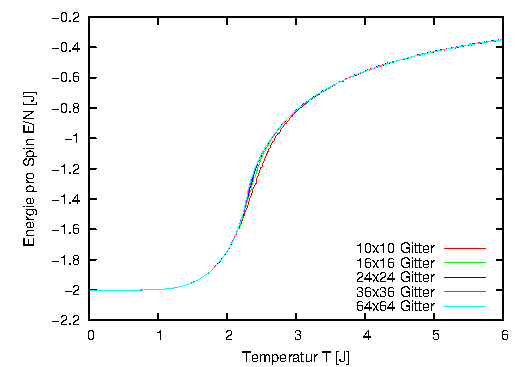
\includegraphics[width=0.48\textwidth]{Diagramme/KMCS/Energie-Temperatur} 
  }
  \subfloat[{\bfseries Mittelwert der W�rmekapazit�t -- Temperatur}]{
    \label{fig:KMCSWaermekapazitaet}
    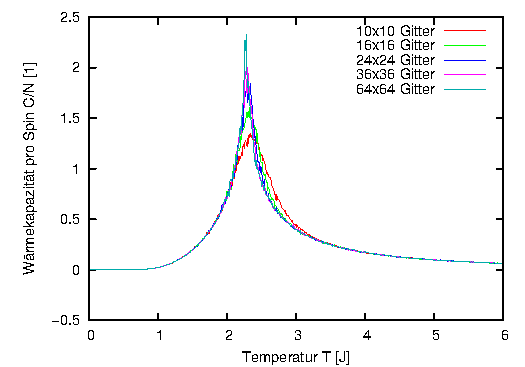
\includegraphics[width=0.48\textwidth]{Diagramme/KMCS/Waermekapazitaet-Temperatur} 
  }
  \caption[Mittelwert der Energie und W�rmekapazit�t -- Temperatur]{Diagramme der Mittelwerte der Energie und W�rmekapazit�t f�r verschieden gro�e Gitter mit periodischen Randbedingungen bei 10000 Messpunkten pro Temperaturpunkt}
  \label{fig:KMCSEnergieWaermekapazitaet}
\end{figure}

Der Mittelwert der Energie (Gl. \ref{eq:Energie}) in Abb. \ref{fig:KMCSEnergie} verl�uft erwartungsgem�� von -2 nach 0. F�r kleine Temperaturen stehen alle Spins in die gleiche Richtung, da die Wahrscheinlichkeit eines Flips (Gl. \ref{eq:Gewicht}) eines einzelnen Spins gegen alle anderen verschwindend gering ist. Weil in einem 2-dimensionalen Gitter mit periodischen Randbedingungen die Anzahl der Kopplungen $N_b=2N$, hat der Mittelwert hier den Wert -2. Je h�her jedoch die Temperatur steigt, je geringer wird der Einfluss des Boltzmanngewichts und f�hrt letztendlich zu einer Gleichverteilung der Spins, die f�r $T\rightarrow\infty$ $\left\langle E/N\right\rangle\rightarrow0$ liefert.

Am Mittelwert der W�rmekapazit�t nach Gl. \ref{eq:Waermekapazitaet} (Abb. \ref{fig:KMCSWaermekapazitaet}), also der Ableitung der mittleren Energie nach $T$, erkennt man deutlich den Phasen�bergang, der sich durch den h�chsten Wert f�r die Steigung der mittleren Energie erkenntlich macht. Da die Gr��e weiterhin die Varianz der Energie darstellt, erkl�hrt sich der Verlauf ebenfalls aus der starken Reaktion der Energie auf geringste Temperatur�nderungen.

Ein Vergleich verschiedener Systemgr��en zeigt eine Verschiebung des Peaks der mittleren W�rmekapazit�t als auch dessen Anwachsen. Verantwortlich hierf�r ist die begrenzte Systemgr��e. Um die reale �bergangstemperatur $T_c$ zu finden, ist ein polynominaler Fit �ber mehrere Systemgr��en hinweg von N�ten (Finite Size Scaling). Auch Verfahren zur Bestimmung der kritischen Exponenten verwenden diese Methode.

\subsection{Autokorrelationszeit der Energie}

Wie wir sehen, nimmt auch die Autokorrelationszeit der Energie $\tau_E$ (Abb. \ref{fig:KMCSAutokorrelationszeitEnergie}, Gl. \ref{eq:Autokorrelationszeit}) um den Phasen�bergang herum stark zu. Das bedeutet, dass die Konfigurationen �ber mehrere MC-Schritte hinweg korrelieren bzw. statistisch abh�ngig sind. Begr�ndet liegt dies in der Tatsache, dass die Korrelationsl�nge $\xi$, ein Ma� f�r die Korrelation innerhalb des Systems, am Phasen�bergang divergiert und die Propagation von Information durch das System viel Zeit ben�tigt. $\tau_E$ ist neben der Temperatur auch vom System insbesondere dessen Gr��e abh�ngig.

\begin{figure}
  \centering
  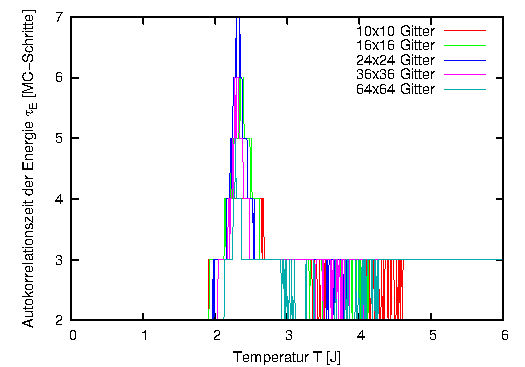
\includegraphics[width=0.48\textwidth]{Diagramme/KMCS/AutokorrelationszeitEnergie-Temperatur} 
  \caption[Autokorrelationszeit der Energie -- Temperatur]{{\bfseries Autokorrelationszeit der Energie -- Temperatur} Diagramm f�r verschieden gro�e Gitter mit periodischen Randbedingungen bei 10000 Messpunkten pro Temperaturpunkt}
  \label{fig:KMCSAutokorrelationszeitEnergie}
\end{figure}

\subsection{Mittelwert der Magnetisierung und Magnetischen Suszeptibilit�t}

\begin{figure}[b!]
  \centering
  \subfloat[{\bfseries Mittelwert der Magnetisierung -- Temperatur}]{
    \label{fig:KMCSMagnetisierung}
    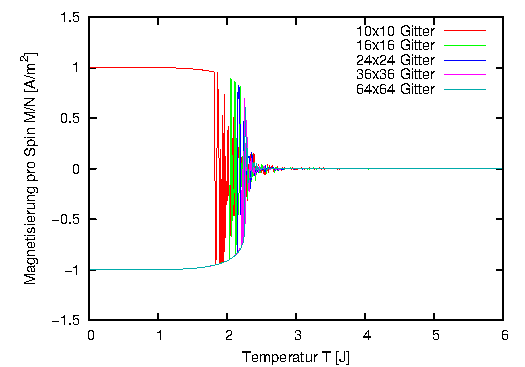
\includegraphics[width=0.48\textwidth]{Diagramme/KMCS/Magnetisierung-Temperatur} 
  }
  \subfloat[{\bfseries Mittelwert der Mag. Suszeptibilit�t -- Temperatur}]{
    \label{fig:KMCSSuszeptibilitaet}
    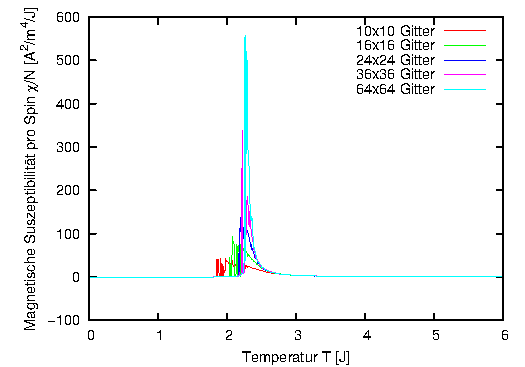
\includegraphics[width=0.48\textwidth]{Diagramme/KMCS/MagnetischeSuszeptibilitaet-Temperatur} 
  }
  \caption[Mittlere Magnetisierung und Magnetische Suszeptibilit�t -- Temperatur]{Diagramme der Mittelwerte der Magnetisierung und Magnetischen Suszeptibilit�t f�r verschieden gro�e Gitter mit periodischen Randbedingungen bei 10000 Messpunkten pro Temperaturpunkt}
  \label{fig:KMCSMagnetisierungUndSuszeptibilitaet}
\end{figure}

Die weiter oben angesprochene Gleichverteilung der Spins bei hohen Temperaturen, dr�ckt sich zus�tzlich in der mittleren Magnetisierung in Abb. \ref{fig:KMCSMagnetisierung} (Gl. \ref{eq:Magnetisierung}) aus. Verringert man von diesem Thermischen Chaos aus die Temperatur, so beginnen die Spins in der N�he des kritischen Punktes, sich in eine Richtung auszurichten. Da hierbei keine der beiden Richtungen einen Vorzug erh�lt, wechselt der Mittelwert der Magnetisierung beliebig das Vorzeichen.

Hier zeigt sich die Simulation mit dem Metropolis Algorithmus (Gl. \ref{eq:KanonischerMetropolis}) fehlerbehaftet, da sich die positiven und negativen Beitr�ge aus Symetriegr�nden aufheben m�ssten. In dieser Phase bilden sich jedoch Cluster von gleich ausgerichteten Spins, die der Algorithmus nur von den R�ndern her beginnen kann umzudrehen, denn das Flippen eine Spins in der Mitte eines solchen Clusters ist sehr unwahrscheinlich. Die Cluster bleiben also f�r l�ngere Zeit bestehen und brechen die Symetrie der Verteilung -- es entsteht eine vermeintliche Magnetisierung. F�r kleine Temperaturen sieht man sogar, dass sich das Vorzeichen garnicht mehr ver�ndert und mit der Zeit alle Spins, die noch entgegen dem Cluster stehen, geflippt werden.

Ein Algorithmus, welcher diesem Sachverhalt Sorge tr�gt, ist z.B. der von Swendson/Wang (1987) und Wolff (1989) \cite{Diplom} erstmals vorgestellte Cluster-Algorithmus. Die Cluster werden analysiert, im Ganzen gewichtet und eventuell geflippt. F�r kleine Temperaturen werden die Cluster also bei fast jedem MC-Schritt geflippt und die Mittelung ergiebt eine verschwindende Magnetisierung.

Die Magnetische Suszeptibilit�t (Abb. \ref{fig:KMCSSuszeptibilitaet}, Gl. \ref{eq:Suszeptibilitaet}) zeigt ein �hnliches Verhalten, wie die W�rmekapazit�t. Auch sie formt zum Phasen�bergang hin einen einen Peak aus. In der Realit�t ist allerdings auch sie immer 0, falls es kein Magnetfeld gibt.

\subsection{Mittelwert der Abs. Magnetisierung und Mag. Suszeptibilit�t}

Nachdem die Magnetisierung zuf�llig das Vorzeichen wechselt und sich f�r Systeme ohne externes Magnetfeld wegmittelt, betrachtet man h�ufig nur die Absolute Magnetisierung (Abb. \ref{fig:KMCSAbsoluteMagnetisierung}) und deren Varianz (Abb. \ref{fig:KMCSAbsoluteSuszeptibilitaet}) aus Gl. \ref{eq:AbsoluteMagnetisierung} und \ref{eq:AbsoluteSuszeptibilitaet}. Beide Gr��en verdeutlichen gut, dass der Prozess vom Thermischen Chaos zur Ordnung hin (und dem ausbilden von Clustern) mit gr��erem System schneller von Statten geht. Da diese spin-inversions-invariant sind, stellen sie trotz Clustern reale Gr��en dar.

Die mittlere Absolute, Magnetische Suszeptibilit�t bietet sich neben der W�rmekapazit�t weiterhin an, $T_c$ und Kritische Exponenten zu finden.

\begin{figure}[bh]
  \centering
  \subfloat[{\bfseries Mittelwert der Abs. Magnetisierung -- Temperatur}]{
    \label{fig:KMCSAbsoluteMagnetisierung}
    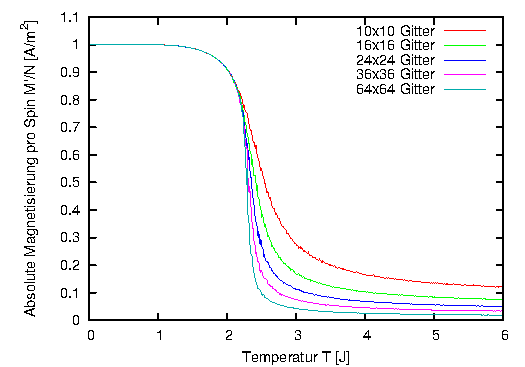
\includegraphics[width=0.48\textwidth]{Diagramme/KMCS/AbsoluteMagnetisierung-Temperatur} 
  }
  \subfloat[{\bfseries Mittelwert der Abs., Mag. Suszeptibilit�t -- Temperatur}]{
    \label{fig:KMCSAbsoluteSuszeptibilitaet}
    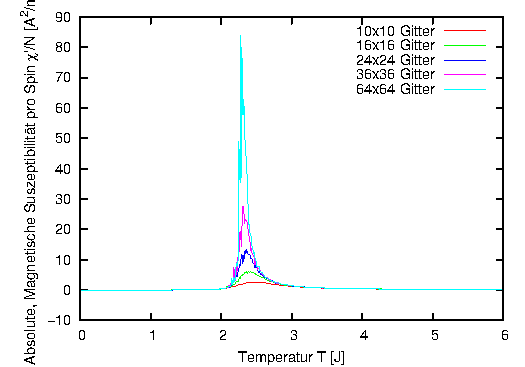
\includegraphics[width=0.48\textwidth]{Diagramme/KMCS/AbsoluteMagnetischeSuszeptibilitaet-Temperatur} 
  }
  \caption[Mittlere Abs. Magnetisierung und Mag. Suszeptibilit�t -- Temperatur]{Diagramme Mittelwerte der der Absoluten Magnetisierung und Magnetischen Suszeptibilit�t f�r verschieden gro�e Gitter mit periodischen Randbedingungen bei 10000 Messpunkten pro Temperaturpunkt}
  \label{fig:KMCSAbsoluteMagnetisierungUndSuszeptibilitaet}
\end{figure}

%TODO:
%            Exact               My              Mean field
%Tc          2.269185            2.26228
%ny          1                   1 (angenommen)  0.5
%gamma       1.75                1.75958         1
%beta        0.125               0.125           0.5

\newpage
\thispagestyle{empty}
\cleardoublepage
\chapter[Quantenmechanische MCS mit Hilfe der Stochastic Series Expansion]{Quantenmechanische MCS\\\LARGE mit Hilfe der Stochastic Series Expansion}
\label{sec:SSE}

Im Folgenden wollen wir uns nun der Simulation des quantenmechanischen Spin-1/2 Heisenberg Systems mithilfe der SSE nach \cite{Buch} und \cite{Sandvik} zuwenden. 

Unsere Beispielapplikation berechnet f�r verschiedene Systeme ({\itshape Offene Kette}, {\itshape Periodische Kette} und {\itshape Periodisches Gitter}) die Energie und die W�rmekapazit�t, wobei wir s�mtliche Daten immer entweder im Vergleich zur {\itshape Exakten Diagonalisierung} des Hamiltonoperators oder entsprechenden Literaturwerten betrachten und einordnen.

\section{Methode}

\subsection{Das Spin-1/2 Heisenberg System}

Der Hamiltonian des Spin-1/2 Heisenberg Systems mit Zeemann-Term ist gegeben durch:

\begin{equation}
H_{\mathrm{Heisenberg}}=\sum_{\left\langle i,j\right\rangle}J_{ij}\cdot\left(S_i^xS_j^x+S_i^yS_j^y+\Delta S_i^zS_j^z\right)-h\sum_{i=0}^{N-1}\mu_{i}\cdot S_i^z
\label{eq:HeisenbergHamiltonian}
\end{equation}

Man betrachtet also eine magnetische Koppelung von 3-dimensionalen, benachbarten Spins (abweichend in $Z$-Richtung um den Faktor $\Delta$) mit der Bindungsmatrix $\boldsymbol{J}$, an denen zus�tzlich ein externes Magnetfeld $\boldsymbol{h}=(0,0,h)^T$ angreift. Das magnetische Moment sei mit $\boldsymbol{\mu}=(0,0,\mu)^T$ benannt.

Das Heisenberg System wird folgenderma�en durch das $\Delta$ klassifiziert:

\begin{itemize}
\item $\Delta<-1$: Ising-Phase
\item $\Delta=-1$: Isotrope ferromagnetische Phase
\item $\vert\Delta\vert<1$: XY-Phase
\item $\Delta=1$: Isotrope antiferromagnetische Phase
\item $\Delta>1$: N\'eel-Phase
\end{itemize}

Wir wollen uns hier speziell mit der isotropen antiferromagnetischen Phase besch�ftigen, wobei wir auch hier wieder alle $J_{ij}=1$ sowie $\mu_i=1$ setzen wollen (Homogenit�t). Die Anordnung betrachten wir weiterhin ohne Magnetfeld ($h=0$). Daraus ergibt sich der vereinfachte Hamiltonian

\begin{equation}
H=\sum_{\left\langle i,j\right\rangle}S_i^xS_j^x+S_i^yS_j^y+S_i^zS_j^z=\sum_{\left\langle i,j\right\rangle}\boldsymbol{S}_i\cdot\boldsymbol{S}_j
\label{eq:BeispielHeisenbergHamiltonian}
\end{equation}

welchen man mit $S_i^\pm=S_i^x\pm iS_i^y$ zu

\begin{equation}
H=\sum_{b=1}^{N_b}\frac{1}{2}\left(S_{i(b)}^+S_{j(b)}^-+S_{i(b)}^-S_{j(b)}^+\right)+S_{i(b)}^zS_{j(b)}^z
\label{eq:BeispielHeisenbergHamiltonianPM}
\end{equation}

umformen kann, wobei wir die P�rchen $\left\langle i,j\right\rangle$ mit einem Index $b$ durchnummerieren und f�r die Spin-Indizes Nachbar-Funktionen $i(b)$ und $j(b)$ einf�hren; diese ergeben sich aus der Geometrie des Systems. Betrachtet man die Spin Operatoren dann in der Standardbasis bez�glich $S^z$, so kann man den Hamiltonian pro Koppelung (engl. Bond) in einen diagonalen $H_{0,b}$ und einen off-diagonalen Teil $H_{1,b}$ aufspalten:

\begin{equation}
H=-\sum_{b=1}^{N_b}\left(\underbrace{\frac{1}{4}-S_{i(b)}^zS_{j(b)}^z}_{H_{0,b}}-\underbrace{\frac{1}{2}\left(S_{i(b)}^+S_{j(b)}^-+S_{i(b)}^-S_{j(b)}^+\right)}_{H_{1,b}}\right) + \left\{\frac{N_b}{4}\right\}
\label{eq:BeispielHeisenbergHamiltonianTeile}
\end{equation}

Hierbei f�gen wir $H_{0,b}$ eine zus�tzliche Konstante $1/4$ ein, um die Eigenwerte des Produktoperators $-S_{i(b)}^zS_{j(b)}^z$ von $\pm1/4$ auf $\{0,\;1/2\}$, was f�r sp�tere Berechnungen bequemer ist.

\subsection{Reihenentwicklung}

Wie beim klassischen Ising Modell im Abschnitt \ref{sec:KlassischesSampling} versuchen wir nun auch, die Zustandssumme durch einen Monte-Carlo Ansatz anzun�hern, anstatt den gesamten Zustandsraum abtasten zu m�ssen. Der obere Ansatz ist hier jedoch nicht hilfreich, weil wir die Energie bzw. den Hamiltonian f�r den Boltzmannfaktor (in der Zustandssumme) nicht berechnen k�nnen. Deshalb schlagen wir einen anderen Weg ein:

Die quantenmechanische Zustandssumme

\begin{equation}
Z=\tr e^{-\beta H}
\label{eq:QuantenmechanischeZustandssumme}
\end{equation}

ist �ber Spur des "`Boltzmann-Operators"' definiert. Schreiben wir die Spur mit der Basis $\vert\alpha\rangle$ und verwenden f�r die Exponentialfunktion die Reihendarstellung, ergibt sich

\begin{align}
Z&=\sum_{n=0}^\infty\frac{(-\beta)^n}{n!}\sum_\alpha\langle\alpha\mid H^n\mid\alpha\rangle\label{eq:QuantenmechanischeZustandssummeReihe}\\
&=\sum_{n=0}^\infty\frac{(-\beta)^n}{n!}\sum_\alpha\langle\alpha\mid\left(-\sum_{b=1}^{N_b}H_{0,b}-H_{1,b}\right)^n\mid\alpha\rangle\label{eq:QuantenmechanischeZustandssummeHEingesetzt}\ \mathrm{,}
\end{align}

wobei wir die obige Gl. \ref{eq:BeispielHeisenbergHamiltonianTeile} f�r den Hamiltonian einsetzen.

An dieser Stelle f�hren wir die Potenzierung der Hamiltonians explizit durch Ausmultiplizieren aus und erhalten dadurch Hamiltonoperatorketten der L�nge $n$, sogenannte Operatorstrings. Jedes Kettenglied ist hierbei entweder diagonal oder off-diagonal und geh�rt zu einer bestimmten Koppelung $\langle i,j\rangle$ mit Index $b$. Da jede m�gliche Kombination von $n$ Operatoren vorkommt, haben wir insgesamt $(2N_b)^n$ Operatorstrings. Um diese geeignet zu verwalten, definieren wir die Menge aller Operatorstrings der L�nge $n$ als $\{S_n\}$ und ordnen jedem String je eine Funktion f�r die beiden Indizes $a(p)\in\{0,1\}$ und $b(p)\in\{1,\ldots,N_b\}$ der Hamiltonoperatoren zu, welche den exakten Operator $H_{a(p),b(p)}$ an der Position $p$ im String darstellen. Dar�ber hinaus hebt sich das erste Minuszeichen vor der Summe mit dem vor dem $\beta$ weg und das Minuszeichen zwischen den Hamiltonoperatoren ziehen wir mit der Anzahl der off-diagonalen Operatoren $n_1$ vor das Matrixelement:

\begin{equation}
Z=\sum_{n=0}^\infty\frac{\beta^n}{n!}\sum_\alpha\sum_{\{S_n\}}(-1)^{n_1}\langle\alpha\mid\prod_{p=0}^{n-1}H_{a(p),b(p)}\mid\alpha\rangle
\label{eq:QuantenmechanischeZustandssummeStrings}
\end{equation}

Nun betrachten wir noch die unendliche Summe �ber $n$. Diese schneiden wir bei $n=L$ ab (eine Fehlerrechnung folgt sp�ter) und bringen alle Operatorstrings mit $n<L$ auf die L�nge $L$, indem wir $L-n$ Einheitsmatrizen in sie einf�gen, die wir sinnvollerweise $H_{0,0}$ nennen. Dies f�hrt zu nur noch {\bfseries einer} Menge von Operatorstrings $S_L$, in die die k�rzeren integriert wurden. Da es aber $\binom{L}{n}$ M�glichkeiten gibt die Einheitsmatrizen einzuf�gen, m�ssen wir zus�tzlich durch diese Vielfachheit teilen, da ein ehemaliger $S_n$ Operatorstring auch zuk�nftig nur einfach in die Zustandssumme eingehen soll:

\begin{equation}
Z=\sum_{\{S_L\}}\frac{\beta^{n}(-1)^{n_1}(L-n)!}{L!}\sum_\alpha\langle\alpha\mid\prod_{p=0}^{L-1}H_{a(p),b(p)}\mid\alpha\rangle
\label{eq:QuantenmechanischeZustandssummeAbschneiden}
\end{equation}

$n$ ist nun nicht mehr die Stringl�nge, sondern die Anzahl der Operatoren ungleich $H_{0,0}$.

Wir wollen nun die Wirkung des Operatorstrings auf die Basis $\vert\alpha\rangle$ betrachten: Diese {\itshape propagierten Zust�nde}

\begin{equation}
\vert\alpha(Q)\rangle=\prod_{p=0}^{Q-1}H_{a(p),b(p)}\mid\alpha\rangle
\label{eq:PropagierteZust�nde}
\end{equation}

sind neue Basiszust�nde, sie ergeben sich also nicht aus der Superposition von anderen Zust�nden. Explizit ist die Wirkung eines diagonalen Operators auf einen Basiszustand

\begin{align}
H_{0,b}\mid\ldots\uparrow_{i(b)}\ldots\uparrow_{j(b)}\ldots\rangle&=\frac{1}{4}-(\frac{1}{2}\cdot\frac{1}{2})=0\ \mathrm{,}\label{eq:DigonalOpAuf11}\\
H_{0,b}\mid\ldots\downarrow_{i(b)}\ldots\downarrow_{j(b)}\ldots\rangle&=\frac{1}{4}-(-\frac{1}{2}\cdot-\frac{1}{2})=0\ \mathrm{,}\label{eq:DigonalOpAuf00}\\
\langle\ldots\uparrow_{i(b)}\ldots\downarrow_{j(b)}\ldots\mid H_{0,b}\mid\ldots\uparrow_{i(b)}\ldots\downarrow_{j(b)}\ldots\rangle&=\frac{1}{4}-(\frac{1}{2}\cdot-\frac{1}{2})=\frac{1}{2}\ \mathrm{,}\label{eq:DigonalOpAuf10}\\
\langle\ldots\downarrow_{i(b)}\ldots\uparrow_{j(b)}\ldots\mid H_{0,b}\mid\ldots\downarrow_{i(b)}\ldots\uparrow_{j(b)}\ldots\rangle&=\frac{1}{4}-(-\frac{1}{2}\cdot\frac{1}{2})=\frac{1}{2}\label{eq:DigonalOpAuf01}
\end{align}

und die Wirkung eines off-diagonalen Operators auf einen Basiszustand

\begin{align}
H_{1,b}\mid\ldots\uparrow_{i(b)}\ldots\uparrow_{j(b)}\ldots\rangle&=\frac{1}{2}(0+0)=0\ \mathrm{,}\label{eq:OffDigonalOpAuf11}\\
H_{1,b}\mid\ldots\downarrow_{i(b)}\ldots\downarrow_{j(b)}\ldots\rangle&=\frac{1}{2}(0+0)=0\ \mathrm{,}\label{eq:OffDigonalOpAuf00}\\
\langle\ldots\downarrow_{i(b)}\ldots\uparrow_{j(b)}\ldots\mid H_{0,b}\mid\ldots\uparrow_{i(b)}\ldots\downarrow_{j(b)}\ldots\rangle&=\frac{1}{2}\ \mathrm{,}\label{eq:OffDigonalOpAuf10}\\
\langle\ldots\uparrow_{i(b)}\ldots\downarrow_{j(b)}\ldots\mid H_{0,b}\mid\ldots\downarrow_{i(b)}\ldots\uparrow_{j(b)}\ldots\rangle&=\frac{1}{2}\ \mathrm{.}\label{eq:OffDigonalOpAuf01}
\end{align}

Dieser Sachverhalt vereinfacht den Algorithmus deutlich. Beim sp�teren Sampling tragen also nur solche Operatorstrings bei, deren Operatoren auf nicht-parallele Spins wirken. Das Matrixelement einer solchen Operation ist au�erdem immer $\frac{1}{2}$ (dies war der Grund f�r die Konstante $1/4$ in $H_{0,b}$ aus Gl. \ref{eq:BeispielHeisenbergHamiltonianTeile}).

Das Gewicht f�r eine beitragende Konfiguration $\sigma$ ist also

\begin{equation}
p(\sigma,S_L)=\left(\frac{\beta}{2}\right)^n\frac{(L-n)!}{L!}
\label{eq:HeisenbergGewichte}
\end{equation}

wobei wir verwenden, dass $n_1$ auf Quadratgittern und Ketten immer gerade ist und deshalb wegf�llt \cite{Sandvik}.

\subsection{Sampling}

Wir wenden nun die {\bfseries Monte-Carlo Methode} auf Operatorstrings anstatt Zust�nden an: Zu Beginn der Simulation gehen wir von einem leeren Operatorstring und einer zuf�lligen Spinanordnung aus und f�hren wie in Kapitel \ref{sec:Ising} MC-Schritte aus. Diese sind unterteilt in ein Diagonal Update, welches diagonale Operatoren in den String ein- und ausbaut und in ein so genanntes off-diagonales Loop Update, welches diagonale zu off-diagonale Operatoren hin- und zur�cktransformiert. Jedes Update muss allerdings darauf achten, dass die oben angegeben Beschr�nkungen nicht verletzt werden:

\begin{itemize}
\item Operatoren d�rfen nicht auf parallele Spin-Paare wirken, ansonsten annihilieren sie den Zustand (lokale Bedingung).
\item Die Periodizit�t $\vert\alpha\rangle=\vert\alpha(0)\rangle=\vert\alpha(L)\rangle$ des Algorithmus' muss gewahrt werden.
\end{itemize}

Das Sampling kann durch Graphiken wie \ref{fig:OffDiagonalNormal} veranschaulicht werden. Die Anfangskonfiguration $\vert\alpha(0)\rangle$ steht hierbei unten und propagiert durch den Operatorstring in den Endzustand $\vert\alpha(L)\rangle=\vert\alpha(0)\rangle$. Operatoren sitzen jeweils auf zwei "`Spin-Bahnen"' und lassen diese entweder unber�hrt (diagonale Operatoren, wei� dargestellt) oder vertauschen deren Ausrichtung (off-diagonale Operatoren, schwarz dargestellt). Reihen ohne Operatoren signalisieren einen $H_{0,0}$ Operator, also eine Einheitsmatrix.

\begin{figure}[thb]
  \centering
  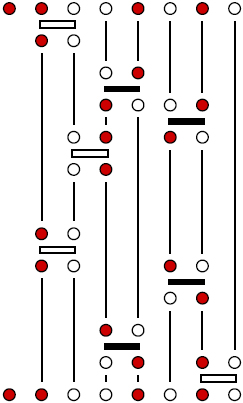
\includegraphics[width=0.3\textwidth]{Images/Off-Diagonal-Normal} 
  \caption[Visualisierung des Operatorstrings; {\itshape Quelle:} \cite{Sandvik}]{{\bfseries Visualisierung des Operatorstrings:} Die Kreise ganz unten und ganz oben stellen die Spinkonfiguration $\vert\alpha(0)\rangle$ bzw. $\vert\alpha(L)\rangle$ dar. Dazwischen liegen diagonale (wei�) und off-diagonale Operatoren (schwarz). Reihen ohne Operatoren signalisieren einen $H_{0,0}$ Operator; {\itshape Quelle:} \cite{Sandvik}}
  \label{fig:OffDiagonalNormal}
\end{figure}

\subsubsection{Diagonales Update}

F�r das Einf�gen von diagonalen Operatoren in den String muss darauf geachtet werden, dass dieser nicht an parallele Spins angelegt wird. Die Periodizit�t hingegen wird durch die Aktion nicht gest�rt, da diagonale Operatoren den Zustand nicht ver�ndern. Das Entfernen von diagonalen Operatoren aus dem Operatorstring ist generell unproblematisch.

Wir legen nun unsere �bergangswahrscheinlichkeiten $\boldsymbol{W}$ f�r das Einf�gen eines Operators an einem Platz $p$ gem�� des {\bfseries Metropolis Algorithmus'} fest (Gl. \ref{eq:Metropolis}):

\begin{equation}
W_{\nu\sigma,\ \mathrm{Einf"ugen}}=\begin{cases}
\frac{p(\sigma,S_L)\cdot N_b}{p(\nu,S_L)}=\frac{\beta N_b}{2(L-n)} & p(\sigma,S_L)\cdot N_b<p(\nu,S_L)\\
1                                                                  & p(\sigma,S_L)\cdot N_b\geq p(\nu,S_L)
\end{cases}
\label{eq:EinfuegeWahrscheinlichkeit}
\end{equation}

Analog erh�lt man beim L�schens eines Operators (ersetzen mit der Einheitsmatrix)

\begin{equation}
W_{\nu\sigma,\ \mathrm{Entfernen}}=\begin{cases}
\frac{p(\sigma,S_L)\cdot N_b}{p(\nu,S_L)}=\frac{2(L-n+1)}{\beta N_b} & p(\sigma,S_L)\cdot N_b<p(\nu,S_L)\\
1                                                                    & p(\sigma,S_L)\cdot N_b\geq p(\nu,S_L)\ \mathrm{.}
\end{cases}
\label{eq:EntferneWahrscheinlichkeit}
\end{equation}

Die Eigenschaft {\itshape Detailed Balance} kann sofort durch Einsetzen in \ref{eq:DetailedBalance} verifiziert werden.

\subsubsection{Off-Diagonales Loop Update}

Beim Austausch von diagonalen und off-diagonalen Operatoren ist der Sachverhalt etwas komplizierter, denn dadurch wird ein Vertauschen von Spinrichtungen (durch den off-diagonalen Operator) hinzugef�gt bzw. entfernt. Es ist selbstverst�ndlich, dass unter der Ber�cksichtigung der Periodizit�t also mindestens zwei off-diagonale Operatoren in solch eine Aktion involviert sein m�ssen. Befinden sich zwischen diesem Operator-Paar allerdings weitere Operatoren, kann es zu einer Regelverletztung der lokalen Bedingung kommen, da ein �ndern der Zust�nde zwischen dem Operatorpaar den dazwischen liegenden beeinflusst (siehe Abb. \ref{fig:Off-Diagonal-Works}). In Abb. \ref{fig:Off-Diagonal-NeedsLoop} wird eine m�gliche L�sung dieses Problems dargestellt; hierbei wird nicht der Zustand zwischen dem Operatorenpaar ver�ndert, sondern der au�erhalb (inklusive dem Anfangs- und Endzustand).

\begin{figure}[thb]
  \centering
  \subfloat[{\bfseries Problematischer (gestrichelt) und Unproblematischer Fall (durchgezogen)}]{
    \label{fig:Off-Diagonal-Works}
    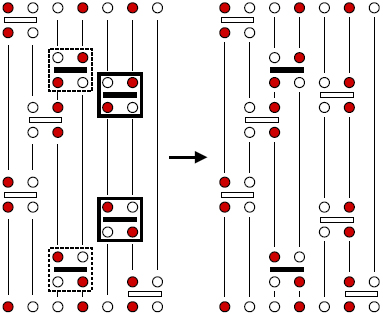
\includegraphics[width=0.41\textwidth]{Images/Off-Diagonal-Works} 
  }\quad\quad
  \subfloat[{\bfseries Ausweg �ber die Modifikation des Anfangszustand}]{
    \label{fig:Off-Diagonal-NeedsLoop}
    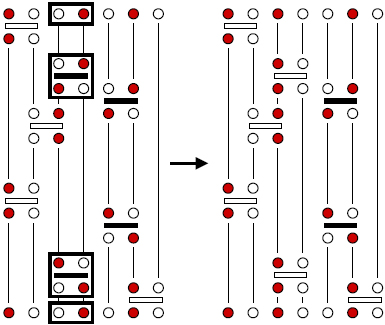
\includegraphics[width=0.41\textwidth]{Images/Off-Diagonal-NeedsLoop} 
  }
  \caption[M�gl. Probleme beim Off-Diagiagonalen Loop Update; {\itshape Quelle:} \cite{Sandvik}]{M�gliche Probleme bzgl. verletzte Bedingungen beim Off-Diagonalen Update. In (a) sehen wir, wie das durchgezogen marktierte Update unproblematisch durchgef�hrt, wobei das gestrichelte Update den Operator zwischen dem Paar so beeinflussen w�rde, dass dieser die lokale Bedingung nicht mehr erf�llt. In (b) sehen wir einen m�glichen Ausweg, da hier Zust�nde zwischen den Operatoren nicht ge�ndert werden, sondern der Anfangs- bzw. Endzustand; {\itshape Quelle:} \cite{Sandvik}}
  \label{fig:ProblematikVonOffDiagonalUpdates}
\end{figure}

Eine andere M�glichkeit w�re nat�rlich, den zweiten (links) anliegenden Spin des involvierten mittleren Operators auch zu �ndern, sodass die lokale Bedingung insgesamt wieder erf�llt ist. Dies beeinflusst aber wieder andere Operatoren, etc.. Im Endeffekt versucht man also, alle sogenannten Loops (siehe Abb. \ref{fig:Off-Diagonal-Loop}), d.h. abgeschlossene Wege durch den Operatorstring, zu finden, da man diese dann wie in Abb. \ref{fig:Off-Diagonal-LoopDone} unabh�ngig von einander flippen kann (Loop Update), wobei Operatoren die ganz in der Loop liegen hin- und sogleich wieder zur�ckgeflippt werden. Der Ausweg in Abb. \ref{fig:Off-Diagonal-NeedsLoop} ist in dieser L�sung inbegriffen, da Loops auch �ber den periodischen Rand hinaus f�hren k�nnen.

\begin{figure}[thb]
  \centering
  \subfloat[{\bfseries Operatorstring mit eingezeichneter Loop}]{
    \label{fig:Off-Diagonal-Loop}
    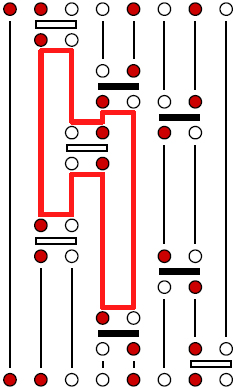
\includegraphics[width=0.3\textwidth]{Images/Off-Diagonal-Loop} 
  }\quad\quad
  \subfloat[{\bfseries Operatorstring nach dem Flippen der Loop}]{
    \label{fig:Off-Diagonal-LoopDone}
    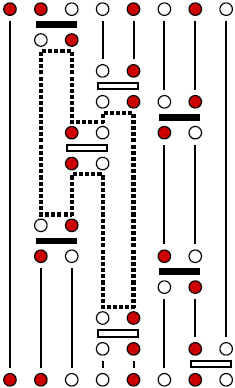
\includegraphics[width=0.3\textwidth]{Images/Off-Diagonal-LoopDone} 
  }
  \caption[Loop im Operatorstring; {\itshape Quelle:} \cite{Sandvik}]{Loop im Operatorstring. (a) bezieht sich noch auf den Ausgangszustand, (b) ergiebt sich nach dem flippen der in (a) angegeben Loop. Operatoren derer beider Seiten am selben Loop liegen werden nicht geflippt (hin und wieder zur�ckgeflippt); {\itshape Quelle:} \cite{Sandvik}}
  \label{fig:LoesungDurchLoopUpdate}
\end{figure}

\subsection{Formeln f�r die mittlere Energie und W�rmekapazit�t}

\subsubsection{Energie}

Augehend von der Gl. \ref{eq:QuantenmechanischeZustandssummeReihe} wollen wir nun eine Formel f�r die mittlere Energie pro Spin $E/N$ herleiten,

\begin{equation}
Z=\sum_{n=0}^\infty\frac{(-\beta)^n}{n!}\sum_{\{\alpha\}_n}\langle\alpha_0\mid H\mid\alpha_{n-1}\cdots\langle\alpha_1\mid H\mid\alpha_0\rangle\ \mathrm{,}
\label{eq:QuantenmechanischeZustandssummeReiheAusgeschrieben}
\end{equation}

wobei in die hintere Summe $n-1$ Summen �ber die Basis eingef�gt wurden. Sodann ergiebt sich der Mittelwert von $E/N$ mit:

\begin{align}
\allowdisplaybreaks
\frac{E}{N}&=\frac{1}{ZN}\sum_{n=0}^\infty\frac{(-\beta)^n}{n!}\sum_{\{\alpha\}_{n+1}}\langle\alpha_0\mid H\mid\alpha_n\cdots\langle\alpha_1\mid H\mid\alpha_0\rangle\label{eq:QuantenEnergie}\\
           &=\frac{1}{ZN}\sum_{n=1}^\infty\frac{(-\beta)^n}{n!}\frac{n}{-\beta}\sum_{\{\alpha\}_n}\langle\alpha_0\mid H\mid\alpha_{n-1}\cdots\langle\alpha_1\mid H\mid\alpha_0\rangle\label{eq:QuantenEnergieSubstitution}
           \displaybreak\\
           &=\frac{1}{ZN}\sum_{n=0}^\infty\frac{(-\beta)^n}{n!}\frac{n}{-\beta}\sum_{\{\alpha\}_n}\langle\alpha_0\mid H\mid\alpha_{n-1}\cdots\langle\alpha_1\mid H\mid\alpha_0\rangle\label{eq:QuantenEnergieMit0}\\
           &=-\frac{\langle n\rangle}{N\beta}\label{eq:QuantenEnergieMittelwert}\\
\left(\frac{E}{N}\right)_{\mathrm{Real}}&=-\frac{\langle n\rangle}{N\beta}+\left\{\frac{N_b}{4N}\right\}\label{eq:QuantenEnergieMitShift}
\end{align}

F�r die erste Gleichheit bemerken wir, dass die letzte Summe nun �ber ein $H$ mehr l�uft. Diese erste Umformung substituiert $n:=n+1$, die zweite f�gt den $n=0$-Term wieder ein, dies ist m�glich, da er ohnehin 0 ergibt. Sodann kann erkannt werden, dass es sich bei dem vorliegenden Ausdruck um den Mittelwert von $n$ handelt. Zu guter Letzt f�gen wir noch die "`verlorene"' Energie-Konstante von Gl. \ref{eq:BeispielHeisenbergHamiltonianTeile} hinzu.

\subsubsection{W�rmekapazit�t}

Die W�rmekapazit�t pro Spin erh�lt man dann �ber die Ableitung der mittleren Energie nach der Temperatur:

\begin{align}
\frac{C}{N}&=\frac{\partial_T E}{N}\\
           &=-\frac{1}{NT}\partial_T \langle n\rangle-\frac{\langle n\rangle}{N}\label{eq:QuantenWaermeKapazitaet}\\
           &=\frac{\langle n^2\rangle-\langle n\rangle^2-\langle n\rangle}{N}\label{eq:QuantenWaermeKapazitaetBest}
\end{align}

\subsection{Cut-Off L}
\label{sec:cutoff}

Da f�r $T\rightarrow\infty$ von $C\rightarrow0$ ausgegangen werden kann, sehen wir, dass $\var n=\langle n\rangle$, das hei�t, der $T$ -- $n$ Graph f�llt in beide Richtungen exponentiell ab. Nach \cite{Sandvik} kann f�r $L$ also ein hinreichend h�herer Wert als $\langle n\rangle$ verwendet werden (ca. $4/3\cdot\langle n\rangle$). Dann erreicht $n$ praktisch nie $L$.

Der Algorithmus muss $L$ also f�r jeden MC-Schritt �berpr�fen und gegebenfalls anpassen.

\section{Implementierung}

Die Struktur der Anwendung ist ebenfalls wieder eng angelehnt an die Beschreibung in \cite{Sandvik}. Der Algorithmus �hnelt dem der klassischen MCS in Abschnitt \ref{sec:KlassischeImplementierung} deutlich, verwendet allerdings andere Messformeln (Gl. \ref{eq:QuantenEnergieMitShift} und \ref{eq:QuantenWaermeKapazitaetBest}) und einen anderen MC-Schritt, da er den Operatorstring inklusive Anfangskonfiguration sampled und nicht nur einzelne Konfigurationen.

\subsection{Initialisierung}

Wie bei der klassischen MCS ben�tigen wir zuerst die Eingabeparameter:

\begin{itemize}
\item Anzahl der Spins $N$
\item Anzahl der Messungen $R_1$
\item Temperatur des Systems $T$
\end{itemize}

Anschlie�end legen wir wieder ein boolsches Array der L�nge $N$ an, welches unseren Anfangszustand $\vert\alpha(0)\rangle$ enth�lt, und initialisieren es mit zuf�lligen Werten. Um den aktuellen Operatorstring abspeichern zu k�nnen, legen wir weiterhin ein Integer-Array $s$ der L�nge $L$ an, welches f�r jeden Platz $p$ im String die Art des Operators (diagonal, off-diagonal oder Einheitsmatrix) -- also $a(p)$ und dessen Position im System $b(p)$ (Koppelung) speichert. Dies k�nnen wir gemeinsam in einer Ganzzahl speichern, wenn wir ausnutzen, dass $a\in\{0,1\}$:

\begin{equation}
s(p)=a(p)+2b(p)
\label{eq:OperatorArrayStorage}
\end{equation}

Wir k�nnen die Informationen aus der Ganzzahl $s(p)$ wieder erhalten, wenn wir pr�fen, ob

\begin{itemize}
\item $s(p)=0 \Rightarrow$ Einheitsmatrix,
\item $\even s(p) \Rightarrow$ Diagonaler Operator,
\item $\odd s(p) \Rightarrow$ Off-diagonaler Operator.
\end{itemize}

Die Position $b(p)$ des Operators erhalten wir, wenn wir mittels einer ganzzahligen Division $b(p)=s(p)/2$. Au�erdem speichern wir die Anzahl der Operatoren $n$, die nicht eine Einheitsmatrix darstellen, da diese Gr��e sp�ter zum Berechnen unserer Messgr��en verwendet wird.

\subsection{Simulation}

F�r jeden MC-Schritt wird zuerst ein Diagonal Update durchgef�hrt und anschlie�end ein Off-Diagonal Loop Update. Abschlie�end wird der Cut-Off $L$ nach Abschnitt \ref{sec:cutoff} eventuell weiter noch oben gesetzt, um dem System genug Freiraum zum Einf�gen weiterer Operatoren zu geben, d.h. wir verl�ngern den Operatorstring, um immer genug Einheitsmatrizen frei f�r diagonale Operatoren zu haben.

\subsubsection{Diagonal Update}

Bei jedem Diagonal Update wird f�r jeden Operatorplatz $p$, auf dem bereits ein diagonaler Operator sitzt, mittels einem Zufallstest entschieden, ob der Operator durch eine Einheitsmatrix ersetzt werden darf. Ist eine Zufallszahl kleiner als die Wahrscheinlichkeit aus Gl. \ref{eq:EntferneWahrscheinlichkeit}, verringert man $n$ um 1 und vermerkt im Operatorstring $s(p)=0$.

Existiert noch kein Operator auf der Position, versucht man einen diagonalen Operator einzuf�gen: Die Koppelung $b$ des Operators wird zuf�llig bestimmt. Wenn die beiden Spins an dieser Koppelung anti-parallel sind, wird mit einem �hnlichen Zufallstest wie oben mit der Wahrscheinlichkeit aus Gl. \ref{eq:EinfuegeWahrscheinlichkeit} entschieden, ob das Einf�gen erfolgt. Als Konsquenz w�rden wir $n$ um 1 erh�hen und $s(p)=2b$ setzen. Um den bis zu $p$ propagierten Zustand $\vert\alpha(p)\rangle$ schnell zu erhalten, schreiben wir ihn in jedem $p$-Schritt mit.

Trifft man auf einen Off-Diagonalen Operator, wird nichts am Operatorstring ver�ndert, lediglich der propagierte Zustand wird angepasst (die beiden Spins tauschen ihren Zustand).

\subsubsection{Off-Diagonal Loop Update}

Um nun die durch das Diagonal Update eingef�gten Operatoren auch in Off-Diagonale Operatoren zu transformieren (oder zur�ck), wird der Operatorstring nun systematisch nach Loops gescannt und f�r jeden Loop wird anschlie�end mit der Wahrscheinlichkeit von 50\% entschieden, diesen gesamten Loop zu flippen.

\paragraph{Die Analyse des Operatorstrings}

Jeder Operator (der keine Einheitsmatrix ist) besitzt vier Vertizes, welche die Ankn�pfungspunkte an die Spin-Bahnen (zwei oben, zwei unten) sind. Diese erhalten nach Abb. \ref{fig:Vertizes} je eine Typnummer $y\in\{0,1,2,3\}$. Mithilfe dieses $y$ und der Position des Operators im String $p$ kann man jeden Vertex global mit der Zahl $v$ indizieren:

\begin{equation}
v(y,p)=v+4p
\label{eq:OperatorVertexStorage}
\end{equation}

Von der Ganzzahl $v$ kann man wie bei \ref{eq:OperatorArrayStorage} wieder auf die speziellen Eigenschaften schlie�en.

\begin{figure}[thb]
  \centering
  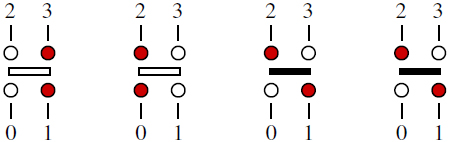
\includegraphics[width=0.4\textwidth]{Images/Vertizes}
  \caption[M�gliche Verwendung der Operatoren mit den Vertex-Typnummern; {\itshape Quelle:} \cite{Sandvik}]{{\bfseries M�gliche Verwendung der Operatoren mit den Typnummern der Vertizes}; {\itshape Quelle:} \cite{Sandvik}}
  \label{fig:Vertizes}
\end{figure}

Nun gehen wir jede Position $p$ im String durch und verkn�pfen Vertizes, die sich auf einer Spin-Bahn gegen�berliegen. Die Verkn�pfungen stellen also die dicken Linien dar, z.B. wie in Abb. \ref{fig:Off-Diagonal-Loop}, die die Operatoren verbinden. D.h. Vertizes stellen die Ecken eines Loop-Gebiets dar, diese Verkn�pfungen und die Operatoren die Kanten. Die Verkn�pfung wird in einem Verkn�pfungs-Array $x$ gespeichert. Zu beachten ist, dass Loops durchaus auch �ber den periodischen Rand hinweg m�glich sind!

\paragraph{Flippen der Loops}

Dieses wird nun St�ck f�r St�ck durchgef�hrt: F�r jede Loop wird mit einer Wahrscheinlichkeit 50\% entschieden, ob diese geflippt werden soll. Ist dies der Fall, geht man auf den Kanten des Loop-Gebiets von Operator zu Operator und flippt einen jeden. Operatoren, die mitten in einer Loop liegen, werden also nicht ver�ndert. Wird eine Loop geflippt, die sich �ber die periodischen R�nder hinaus erstreckt, muss anschlie�end der Anfangszustand demensprechend ver�ndert werden.

\subsection{Analyse}

Die abgespeicherten Werte f�r $n$ werden nach der Simulation verwendet, um sie -- wie in Abschnitt \ref{sec:Autokorrelation} erkl�rt -- zu analysieren. Ihre Anwendung zur Berechnung der Gr��en {\bfseries Energie} und {\bfseries W�rmekapazit�t} werden in den Gleichungen \ref{eq:QuantenEnergieMitShift} und \ref{eq:QuantenWaermeKapazitaetBest} beschrieben.

\subsection{Quellcode}

Der vom Author geschriebene C++ Quellcode ist im Anhang \ref{sec:code} zu finden. Folgende Dateien sind f�r diese quantenmechanische Simulation relevant:

\begin{itemize}
\item\ref{code:SIM}: Hauptprogramm SIM
\item\ref{code:AbstractLattice}: Abstrakte Gitterklasse
\item\ref{code:Open1DLattice}: 1D Kette mit offenen Randbedingungen
\item\ref{code:Periodic1DLattice}: 1D Kette mit periodischen Randbedingungen
\item\ref{code:Periodic2DLattice}: 2D Gitter mit periodischen Randbedingungen
\item\ref{code:AbstractAlgorithm}: Abstrakte Algorithmusklasse
\item\ref{code:SSEAlgorithm}: SSE Algorithmus
\item\ref{code:AbstractAnalyzer}: Abstrakte Analyseklasse
\item\ref{code:SseEnergyAnalyzer}: Analyse f�r die Energie (SSE)
\item\ref{code:SseHeatCapacityAnalyzer}: Analyse f�r die W�rmekapazit�t (SSE)
\end{itemize}

\section{Ergebnisse und Diskussion}

Im Folgenden sind die Messergebnisse der SSE-Simulationen aufgef�hrt. Bis auf die explizite Erw�hnung im ersten Unterabschnitt wurde auf eine Fehlerdarstellung in den Diagrammen verzichtet, da die Fehler ihrer (kleinen) Gr��e wegen nicht darstellbar waren.

\subsection{Heisenbergkette mit periodischen Randbedingungen}

Auf den Abbildungen \ref{fig:KettenEnergieTemperatur} und \ref{fig:KettenWaermekapazitaetTemperatur} sieht man die mittlere Energie und die mittlere W�rmekapazit�t f�r verschieden gro�e Systeme (periodische Ketten) aufgetragen. Diese Kurven verlaufen stets �bereinander, da im 1-dimensionalen Fall noch kein Phasen�bergang auftritt. Das System befindet sich also entweder nahe dem Grundzustand oder besitzt bereits eine so geringe Korrelationsl�nge, dass f�r verschiedene Gr��en keine Effekte auftreten (vgl. Er�rterung in \ref{sec:IsingEnergie}). Die jeweils gleiche Grundzustandsenergie von $-0.4432$ stimmt sehr gut mit dem in \cite{Diplom} auf Seite 58 angegeben Wert �berein.

\begin{figure}[bth]
  \centering
  \subfloat[{\bfseries Mittelwerte der Energie}]{
    \label{fig:KettenEnergieTemperatur}
    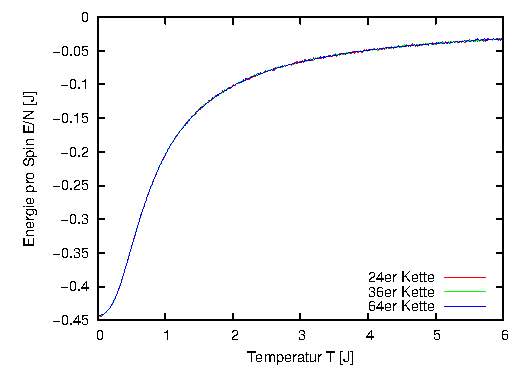
\includegraphics[width=0.48\textwidth]{Diagrams/SSE/Chain_Energy-Temperature} 
  }
  \subfloat[{\bfseries Mittelwerte der W�rmekapazit�t}]{
    \label{fig:KettenWaermekapazitaetTemperatur}
    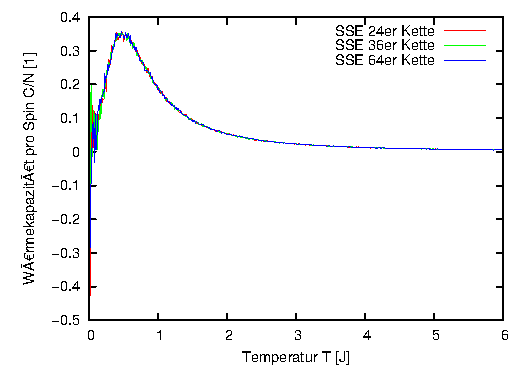
\includegraphics[width=0.48\textwidth]{Diagrams/SSE/Chain_SpecificHeat-Temperature} 
  }
  \caption[Mittelwerte der Energie und W�rmekapazit�t; {\itshape Quelle:} Eigenwerk]{Mittelwerte der Energie und W�rmekapazit�t f�r verschiedene Systemgr��en einer periodischen Kette bei 100000 Messpunkten pro Temperaturpunkt; {\itshape Quelle:} Eigenwerk}
  \label{fig:KettenEnergieWaermekapazitaet}
\end{figure}

Wir betrachten nun noch explizit den absoluten Fehler (Standardabweichung) in Abb. \ref{fig:KettenFehlerEnergie}: Mit steigender Systemgr��e tritt also ein immer st�rker Effekt zu Tage; bei hohen Temperaturen gibt es wesentlich mehr m�gliche Konfigurationen. All diese Konfigurationen haben eine �hnliche Energie und m�ssen gesampelt werden. Bei $T=0$ muss das System nur zum Grundzustand finden.

\begin{figure}
  \centering
  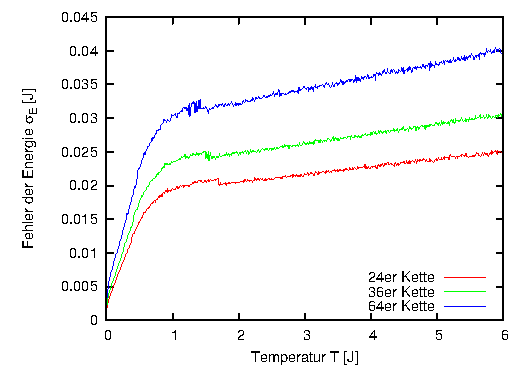
\includegraphics[width=0.48\textwidth]{Diagrams/SSE/Chain_ErrorEnergy-Temperature} 
  \caption[Absoluter Fehler der Energie; {\itshape Quelle:} Eigenwerk]{{\bfseries Absoluter Fehler der Energie} f�r verschiedene Systemgr��en einer periodischen Kette bei 100000 Messpunkten pro Temperaturpunkt; {\itshape Quelle:} Eigenwerk}
  \label{fig:KettenFehlerEnergie}
\end{figure}

\subsection{Heisenberggitter mit periodischen Randbedingungen}

Nach Korrolar 1.11 aus \cite{Branch} besitzt das 2-dimensionale Gitter im Gegensatz zum 1D-Fall einen Phasen�bergang, d.h. zur Temperatur $T_c$ hin divergiert die Korrelationsl�nge und damit die Gr��e der Wei�schen Bezirke (Cluster), so dass in der Umgebung um diesen kritischen Punkt die Gr��e des Systems eine gravierende Rolle spielt. Beide Grundzustandsenergien, -0.67887 und -0.702, werden durch \cite{Scaling} best�tigt.

\begin{figure}[bh]
  \centering
  \subfloat[{\bfseries Mittelwerte der Energie}]{
    \label{fig:GitterEnergieTemperatur}
    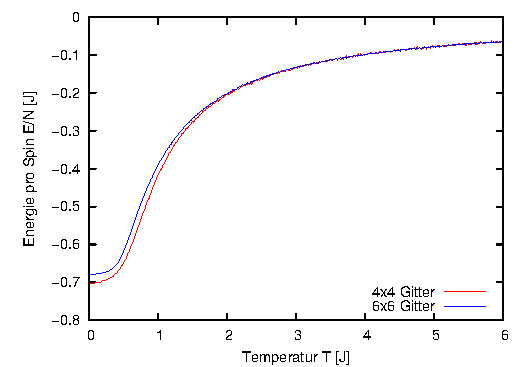
\includegraphics[width=0.48\textwidth]{Diagrams/SSE/Lattice_Energy-Temperature} 
  }
  \subfloat[{\bfseries Mittelwerte der W�rmekapazit�t}]{
    \label{fig:GitterWaermekapazitaetTemperatur}
    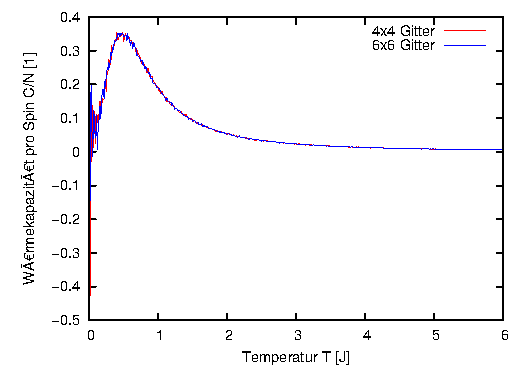
\includegraphics[width=0.48\textwidth]{Diagrams/SSE/Lattice_SpecificHeat-Temperature} 
  }
  \caption[Mittelwerte der Energie und W�rmekapazit�t; {\itshape Quelle:} Eigenwerk]{Mittelwerte der Energie und W�rmekapazit�t f�r verschiedene Systemgr��en eines periodischen Gitters bei 100000 Messpunkten pro Temperaturpunkt; {\itshape Quelle:} Eigenwerk}
  \label{fig:ModellEnergieWaermekapazitaet}
\end{figure}

\subsection{Vergleich verschiedener Modelle / Exakte Diagonalisierung}

In den Abbildungen \ref{fig:AlleEnergieTemperatur} und \ref{fig:AlleWaermekapazitaetTemperatur} sind die Energie und die W�rmekapazit�t f�r die drei betrachteten Modelle (Kette mit offenen, Kette mit periodischen und Gitter mit periodischen Randbedingungen) aufgetragen. Die exakte, dunklere Linie beschreibt die Werte der ED-Methode {\itshape(Exakte Diagonalisierung)}.

Die Energiekurven zeigen im 1-dimensionalen Fall keinen sichtbaren Unterschied zwischen den Methoden SSE und ED, wohingegen die SSE-Werte f�r das Gitter eine gut sichtbare h�here Ungenauigkeit aufweisen. Die Differenz der Grundzustandsenergien erkl�ren sich wohl Haupts�chlich durch die gr��ere Anzahl von Koppelungen pro Spin, qualitativ zeigen die Kurven allerdings ebenfalls kaum Unterschiede.

Die Ableitung der Energie nach der Temperatur, die W�rmekapazit�t, ist wie erwartet deutlich ungenauer. Besonders in den Temperaturen nahe 0 spielen arithmetische Fehler der Implementierung (Maschinengenauigkeit) eine gro�e Rolle, da dort gro�e Zahlen subtrahiert werden. Auffallend ist, dass die beiden periodischen Modelle diesselbe maximale W�rmekapazit�t besitzen.

\begin{figure}[bh]
  \centering
  \subfloat[{\bfseries Mittelwerte der Energie}]{
    \label{fig:AlleEnergieTemperatur}
    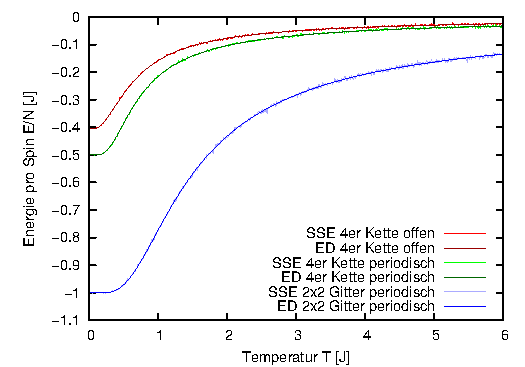
\includegraphics[width=0.48\textwidth]{Diagrams/SSE/All_Energy-Temperature} 
  }
  \subfloat[{\bfseries Mittelwerte der W�rmekapazit�t}]{
    \label{fig:AlleWaermekapazitaetTemperatur}
    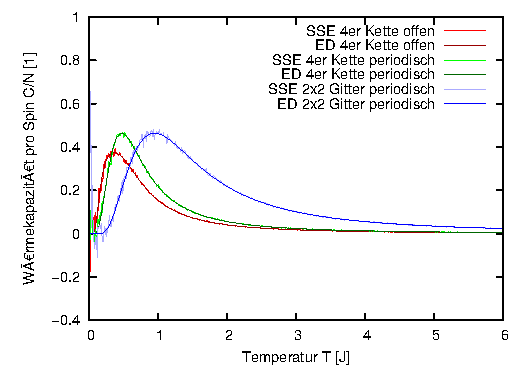
\includegraphics[width=0.48\textwidth]{Diagrams/SSE/All_SpecificHeat-Temperature} 
  }
  \caption[Mittelwerte der Energie und W�rmekapazit�t; {\itshape Quelle:} Eigenwerk]{Mittelwerte der Energie und W�rmekapazit�t f�r die verschiedenen Modelle 1D-Offen, 1-Periodisch und 2D-Periodisch mit der Spinanzahl 4 bei 100000 Messpunkten pro Temperaturpunkt; {\itshape Quelle:} Eigenwerk}
  \label{fig:AlleEnergieWaermekapazitaet}
\end{figure}

An dem Beispiel der 4 Spin langen Heisenbergkette mit offenen Randbedingungen, wollen wir uns nun noch die Verwendung der Exakten Diagonalisierung veranschaulichen \cite{Ham}:

Da der Hamiltonian jeden Unter-Zustandsraum $\Omega_i$ aller Basiszust�nde diesselbe Anzahl $i$ aufw�rtsgerichteter Spins (siehe \cite{Spincount}) stabil l�sst (Erhaltung der Summe aller $S_j^z$), stellt er in einer geeignet sortierten Basis eine Blockmatrix dar:

\tiny
\[
H=\left(\begin{blockarray}{cccccccccccccccc}
\begin{block}{\{c\}ccccccccccccccc}
0.75  &&&&&&&&&&&&&&& 0\\
\end{block}
\begin{block}{c\{cccc\}ccccccccccc}
& 0.25  & 0.5   & 0     & 0     \\
& 0.5   & -0.25 & 0.5   & 0     \\
& 0     & 0.5   & -0.25 & 0.5   \\
& 0     & 0     & 0.5   & 0.25  \\
\end{block}
\begin{block}{ccccc\{cccccc\}ccccc}
&&&&& 0.25  & 0.5   & 0     & 0     & 0     & 0     \\
&&&&& 0.5   & -0.75 & 0.5   & 0.5   & 0     & 0     \\
&&&&& 0     & 0.5   & -0.25 & 0     & 0.5   & 0     \\
&&&&& 0     & 0.5   & 0     & -0.25 & 0.5   & 0     \\
&&&&& 0     & 0     & 0.5   & 0.5   & -0.75 & 0.5   \\
&&&&& 0     & 0     & 0     & 0     & 0.5   & 0.25  \\
\end{block}
\begin{block}{ccccccccccc\{cccc\}c}
&&&&&&&&&&& 0.25  & 0.5   & 0     & 0     \\
&&&&&&&&&&& 0.5   & -0.25 & 0.5   & 0     \\
&&&&&&&&&&& 0     & 0.5   & -0.25 & 0.5   \\
&&&&&&&&&&& 0     & 0     & 0.5   & 0.25  \\
\end{block}
\begin{block}{ccccccccccccccc\{c\}}
0&&&&&&&&&&&&&&& 0.75  \\
\end{block}
\end{blockarray}\right)
\]
\normalsize

Die Bl�cke k�nnen nun einzeln diagonalisiert werden, was einen deutlichen Performancegewinn gegen�ber einer gesamten Diagonalisierung darstellt. Die Eigenwerte der obigen Matrix sind \{0.75, 0.75, 0.75, 0.75, 0.75, 0.457107, 0.457107, 0.457107, 0.116025, -0.25, -0.25, -0.25, -0.957107, -0.957107, -0.957107, -1.61603\}. Mithilfe dieser k�nnen nun z.B. die Boltzmanngewichte bzw. die Zustandssumme berechnet werden.

\newpage
\thispagestyle{empty}
\cleardoublepage
\chapter{Zusammenfassung}

Die {\bfseries Stochastic Series Expansion} stellt ein m�chtiges Werkzeug f�r das Sampling von Operatorstrings innerhalb eines quantenmechanischen L�sungsansatzes dar. Sie ist f�r gr��ere 2-dimensionale Systeme der schnellste Weg, um die typischen, thermodynamischen Gr��en zu messen und wird hierf�r an mehreren Instituten erfolgreich eingesetzt. Der Algorithmus ist relativ leicht zu implementieren und arbeitet �u�erst speichersparend.

Im Rahmen dieser Arbeit wurde ein Simulationsprogramm geschrieben, welches nicht nur ein blo�es SSE Modul enth�lt, sondern die M�glichkeit anbietet, die SSE-Daten f�r kleine Systeme mit ED {\bfseries Exakt Diagonalisation} zu �berpr�fen, als auch ein Zusatzmodul f�r das numerische L�sen des klassischen Ising-Modells enth�lt. Nach einem Baukasten Prinzip wurden Klassendateien f�r verschiedene Szenarien hinzugef�gt. So ist die Analyse der Daten in einzelne Pakete gekapselt, um ein H�chstma� an Flexibilit�t zu garantieren. Das Messen einer Gr��e kann also einfach ein- und ausgeschaltet werden. Weiterhin bietet die Anwendung verschiedene Geometriemodelle an, aus denen das gew�nschte gew�hlt werden kann (Periodische Gitter und Offene und Periodische Ketten). Nat�rlich ist es ohne Weiteres m�glich einfach weitere Features hinzuzuf�gen!

Die durchgef�hrten Messungen best�tig die Theorie und liefern sehr genaue Ergebnisse. �ber den Parameter "`measureCount"' kann die Anzahl der durchzuf�hrenden Messungen modifiziert werden. So ist eine Entscheidung zwischen ben�tigter Rechenzeit und Genauigkeit m�glich.

\appendix

\chapter{Quellcode}
\label{sec:code}

\section{Hauptprogramm SIM}

\cppcodefile[label=code:SIM]{SIM.cpp}

\section{Gitter Klassen}

\subsection{Abstrakte Gitter}

\cppcodefile[label=code:AbstractLattice]{Classes/Lattice/AbstractLattice.cpp}

\subsection{1D Gitter mit offenen Randbedingungen}

\cppcodefile[label=code:Open1DLattice]{Classes/Lattice/Open1DLattice.cpp}

\subsection{1D Gitter mit periodischen Randbedingungen}

\cppcodefile[label=code:Periodic1DLattice]{Classes/Lattice/Periodic1DLattice.cpp}

\subsection{2D Gitter mit periodischen Randbedingungen}

\cppcodefile[label=code:Periodic2DLattice]{Classes/Lattice/Periodic2DLattice.cpp}

\section{Algorithmus Klassen}

\subsection{Abstrakter Algorithmus}

\cppcodefile[label=code:AbstractAlgorithm]{Classes/Algorithm/AbstractAlgorithm.cpp}

\subsection{ED}

\cppcodefile[label=code:EDAlgorithm]{Classes/Algorithm/EDAlgorithm.cpp}

\subsection{ISING}

\cppcodefile[label=code:ISINGAlgorithm]{Classes/Algorithm/ISINGAlgorithm.cpp}

\subsection{SSE}

\cppcodefile[label=code:SSEAlgorithm]{Classes/Algorithm/SSEAlgorithm.cpp}

\section{Analysemodule}

\subsection{Abstraktes Analysemodul}

\cppcodefile[label=code:AbstractAnalyzer]{Classes/Analyzer/AbstractAnalyzer.cpp}

\subsection{Analysemodul f�r die Energie (Ising)}

\cppcodefile[label=code:IsingEnergyAnalyzer]{Classes/Analyzer/IsingEnergyAnalyzer.cpp}

\subsection{Analysemodul f�r die W�rme Kapazit�t (Ising)}

\cppcodefile[label=code:IsingHeatCapacityAnalyzer]{Classes/Analyzer/IsingHeatCapacityAnalyzer.cpp}

\subsection{Analysemodul f�r die Magnetisierung (Ising)}

\cppcodefile[label=code:IsingMagnetisationAnalyzer]{Classes/Analyzer/IsingMagnetisationAnalyzer.cpp}

\subsection{Analysemodul f�r die Magnetische Suszeptibilit�t (Ising)}

\cppcodefile[label=code:IsingSusceptibilityAnalyzer]{Classes/Analyzer/IsingSusceptibilityAnalyzer.cpp}

\subsection{Analysemodul f�r die Abs. Magnetisierung (Ising)}

\cppcodefile[label=code:IsingAbsoluteMagnetisationAnalyzer]{Classes/Analyzer/IsingAbsoluteMagnetisationAnalyzer.cpp}

\subsection{Analysemodul f�r die Abs., Mag. Suszeptibilit�t (Ising)}

\cppcodefile[label=code:IsingAbsoluteSusceptibilityAnalyzer]{Classes/Analyzer/IsingAbsoluteSusceptibilityAnalyzer.cpp}

\subsection{Analysemodul f�r die Energie (SSE)}

\cppcodefile[label=code:SseEnergyAnalyzer]{Classes/Analyzer/SseEnergyAnalyzer.cpp}

\subsection{Analysemodul f�r die W�rme Kapazit�t (SSE)}

\cppcodefile[label=code:SseHeatCapacityAnalyzer]{Classes/Analyzer/SseHeatCapacityAnalyzer.cpp}

%=======================================

\let\listfigurenamePARENT\listfigurename
\renewcommand{\listfigurename}{\addcontentsline{toc}{chapter}{\listfigurenamePARENT}\listfigurenamePARENT}
\begingroup
\renewcommand*{\addvspace}[1]{}
\listoffigures
\endgroup

\newpage
\thispagestyle{empty}
\cleardoublepage
\renewcommand{\lstlistlistingname}{\addcontentsline{toc}{chapter}{Quellcodeverzeichnis}Quellcodeverzeichnis}
\lstlistoflistings

\newpage
\thispagestyle{empty}
\cleardoublepage
\let\bibnamePARENT\bibname
\renewcommand{\bibname}{\addcontentsline{toc}{chapter}{\bibnamePARENT}\bibnamePARENT}
\bibliographystyle{alphadin}
\bibliography{Literatur}

\newpage
\thispagestyle{empty}
\cleardoublepage
\chapter*{Erkl�rung zur Selbstst�ndigkeit}
\addcontentsline{toc}{chapter}{Erkl�hrung zur Selbstst�ndigkeit}

Hiermit versichere ich, dass ich diese Arbeit selbstst�ndig verfasst und keine anderen als die angegebenen Quellen und Hilfsmittel benutzt habe.

\vspace{10mm}
\begin{tabular}{@{}p{40mm}@{\hspace{1mm}}l@{\hspace{1mm}}p{30mm}@{\hspace{6mm}}p{50mm}}
\hrule&,&\hrule&\hrule\\[-3mm]
Ort&&Datum&Unterschrift\\
\end{tabular}

\end{document}